\documentclass[a4paper, oneside, table]{memoir}

%% Language and font encodings
\usepackage[english]{babel}

%%% Margins
\setulmarginsandblock{2cm}{2cm}{*}
\setlrmarginsandblock{3cm}{3cm}{*}
\checkandfixthelayout

%% Useful packages
\usepackage{amsmath}
\usepackage{bm}
\usepackage{graphicx}
\usepackage[colorinlistoftodos]{todonotes}
\usepackage[colorlinks=true, allcolors=blue, pdfencoding=auto]{hyperref}
\usepackage{siunitx}
\usepackage{booktabs}
\usepackage[version=4]{mhchem}
\usepackage{listings}

% some commands for making tables with alternating colors (replaces tabular environment)
\definecolor{tablegrey}{gray}{0.9}
\let\oldtabular\tabular
\let\endoldtabular\endtabular
\renewenvironment{tabular}{\rowcolors{2}{white}{tablegrey}\oldtabular}{\endoldtabular}
\def\arraystretch{1.2}

%% TIKZ
\usetikzlibrary{quotes,angles}

%% Bibliography
\usepackage[numbers]{natbib}

\author{Tim Birger Tejsner}
\title{Oxygen Dynamics in the High-Temperature Superconductor LSCO+O}
\date{\today}

%\includeonly{ch/simulation}

\begin{document}
%\maketitle
\tableofcontents

\clearpage

\listoffigures
\listoftables
\listoftodos

\chapter{Introduction}

In this thesis, we explore certain aspects of the so-called high-temperature superconductors. While these materials were discovered fairly recently (1986), they have a rich history with hundreds of thousands of citations and, to this day, a lively debate surrounding the microscopic nature of this mysterious macroscopic quantum state. The purpose of this chapter is to briefly state the `the story so far' in broad strokes, and then dive deeper into state-of-the-art research relevant for the work performed in this thesis.

\section{Superconductivity}
Superconductivity is a state of matter where a material is able to conduct electricity with \emph{zero} resistance below a certain critical temperature $T_\text{c}$. Since we, fortunately, live in a world where the `spherical cow in a vacuum' model does not apply, it is remarkable to find \emph{real} materials where electrons can propagate without friction. In fact, experiments have shown, that under the right conditions it is possible to keep a persistent superconducting current running for 100000 years \cite{File1963}!

Superconductivity was first discovered in 1911 by Kamerlingh Onnes, essentially as a consequence of being able to liquefy helium in 1908 and reach temperatures close to absolute zero (see \cite{VanDelft2010} and references therein for a breakdown of the experiments). His low-temperature measurement of lead revealed a sudden drop in resistivity at \SI{4.2}{\kelvin}, as seen in the historic plot on figure \ref{fig:onnes}

\begin{figure}
    \centering
    \includegraphics[width=\textwidth]{fig/intro/onnes.png}
    \caption{\textbf{Left}: Kammerling Onnes (right) and his chief engineer (left) in their cryogenics lab. \textbf{Right}: Resistivity as a function of temperature in elemental Lead. Both images from \cite{VanDelft2010}.}
    \label{fig:onnes}
\end{figure}

\begin{figure}
    \centering
    \missingfigure{Meissner effect}
    \caption{Meissner effect}
    \label{fig:meissner}
\end{figure}

Despite this remarkable experimental result, it would be 20 years for the next major milestone to appear. In 1933 the Meissner effect was discovered \cite{Meissner1933}, showing that superconducting materials would completely resist applied magnetic field by exhibiting perfect diamagnetism as sketched in figure \ref{fig:meissner}. In 1935 this effect was phenomenologically explained by the London equations, showing that the Meissner effect is due to superconducting currents on the surface of the material \cite{London1935}. From their relatively simple set of equations, an observable length scale known as the penetration depth was defined
%
\[ \lambda_\text{L} = \sqrt{\frac{m}{\mu_0 n q^2}} \, \]
%
where $\mu_0$ is the permeability of free space, $n$ the number concentration of the superconducting carriers, $m$ the electron mass and $q$ the electron charge. This length scale determines how an external magnetic field penetrates the superconductor through the relationship $B(x) = B(0) \exp (-x / \lambda)$. $\lambda$ is typically on the order of \SIrange{20}{100}{\nano\meter} \cite{Kittel2005}.

Another roughly 20 years would pass until Landau's work on phase transitions paved the way to understanding the superconducting phase transition as a thermodynamic quantity through the Ginzburg-Landau equations in 1950 \cite{Ginzburg2009}. I will not repeat the details here, but the idea is to make a polynomial expansion of the free energy as a function of a complex superconducting wavefunction $\psi$. As the material is cooled below $T_\text{c}$, $\psi$ `choses' a phase and breaks gauge symmetry, analogous to how a ferromagnet choses a common direction for the magnetic moment at the magnetic phase transition. This description predicts an new characteristic length scale of the superconductor called the \emph{coherence length} $\xi$ and recasts the penetration depth in terms of $\psi$:
%
\[ \xi = \sqrt{\frac{\hbar^2}{4m|\alpha|}} \qquad \lambda = \sqrt{\frac{m}{4\mu_0 e^2 \psi_0^2 }} \, , \]
%
where $\alpha$ is a phenomenological parameter of the polynomial expansion. The ratio of these parameters, $\kappa = \lambda / \xi$, are used to classify superconductors into type-I ($\kappa < 1 / \sqrt{2}$) and type-II ($\kappa > 1 / \sqrt{2}$). The significance of $\kappa > 1 / \sqrt{2}$ can be understood as a threshold where the surface tension between normal and superconducting phases becomes negative \cite{Abrikosov1957}. Intuitively, the coherence length $\xi$ defines the shortest length within which the superconducting carrier concentration are allowed to change considerably. For elemental metals $\xi$ can be on the nanometre to micrometre scale: \SI{1600}{\nano\meter} in Al and \SI{83}{\nano\meter} in Pb \cite{Kittel2005}. In the cuprates (which will be discussed in detail in the next section), $\xi$ is typically on the order of a few lattice spacings (\SI{1}{\nano\meter} in YBa$_2$Cu$_3$O$_{7-\delta}$ \cite{Tomimoto1999}).

Based on Ginzburg-Landau theory, \citeauthor{Abrikosov1957} predicted the existence of vortices in Type-II superconductors, which showed excellent agreement with the measured magnetization of several lead alloys \cite{Abrikosov1957}. These vortices can be pinned by defects and form a lattice that we have been able to image using modern day microscopy techniques (see e.g. \cite{Wells2015} for a recent example with beautiful real-space images). The experimental evidence piled up \cite{Doll1961, Deaver1961}, and it quickly became evident that Ginzburg-Landau theory is applicable to most known superconductors, including the cuprates and iron-based varieties.

Despite the descriptive power of Ginzburg-Landau theory, we are left with no recipe on how to construct, even theoretically, `better' superconductors. In order to manipulate material properties, it is necessary to understand the microscopic properties that lead to macroscopic behaviour (e.g. how phonons influence thermal properties or how magnetic exchange influence magnetic properties. Inspired by Ginzburg-Landau theory, rapid progress towards a microscopic theory was being made in the mid 1950s, culminating in the famous BCS theory formulated by Bardeen, Cooper and Schrieffer \cite{Bardeen1957}. 

BCS theory is based on the assumption that an attractive interaction between electrons at the Fermi level can result in so-called `cooper-pairs', a bosonic quasi-particle consisting of an electron pair of opposite momentum and spin. The bosonic nature of this quasi-particle can, at low temperatures, result in a Bose-Einstein condensate where a large fraction of these electron pairs occupy the lowest energy quantum state. This microscopic theory of superconductivity made several testable predictions, such as the appearance of an energy gap with a temperature-dependent width $\Delta(T)$ in the electronic density of states related to the critical temperature through the relationship
%
\[ 2\Delta(T=0) = 3.5 k_\text{B} T_\text{c} \, , \]
%
where $k_\text{B}$ is the Boltzmann constant. A few years later electron tunnelling experiments confirmed this prediction with reasonable accuracy \cite{Giaever1960, Giaever1960a}. Additionally, \citeauthor{Josephson1962} predicted that superconducting currents could tunnel across an insulating a barrier \cite{Josephson1962}, experimentally verified a few years later \cite{Jaklevic1965}.

While BCS theory predicts an attractive interaction between electrons, the original paper \cite{Bardeen1957} makes no assumption about the nature of this interaction. Some experiments, performed a few years prior, showed that $T_\text{c}$ of Hg$^{198}$ was higher when compared to that of natural Hg (avg. atomic weight of 200.6) \cite{Maxwell1950, Reynolds1950}. Since the chemistry of these materials can be assumed identical, this experiment suggests a positive correlation between phonon frequencies and $T_\text{c}$, since lighter elements have more energetic vibrations. Assuming an attractive potential due to lattice vibrations, BCS theory could relate the attractive interaction to phonon frequencies and predict a relative relationship between isotopic mass and critical temperature \cite{DeLaunay1954}:
%
\[ T_\text{c} \propto \frac{1}{\sqrt{m_\text{ion}}} \, , \]
%
where $m_\text{ion}$ is the isotopic mass of the constituent ionic species. With BCS theory, superconductivity in many elemental metals were believed to be `solved' with the identification of phonon-mediated superconductivity. Unfortunately, this discovery also set a \emph{practical} upper limit on $T_\text{c}$. In order to increase phonon frequencies, and thus critical temperatures, we need materials with low mass atomic species, while still being crystalline. At ambient pressure this practical upper limit is often quoted to be around \SI{30}{\kelvin}. A good demonstration of this principle is actually a counter-example where researchers were able to reach a critical temperature of $T_\text{c} = \SI{200}{\kelvin}$ by applying a pressure of \SI{155}{\giga\pascal} to H$_2$S \cite{Drozdov2015}. This material contains the light atomic species we require, but cannot crystallize at ambient pressures so we can only reach high critical temperatures under extreme conditions. A different example is the highly unusual case of MgB$_2$, where coincidences add up to an unusually high electron-phonon coupling resulting in a critical temperature of $T_\text{c} = \SI{39}{\kelvin}$ \cite{Nagamatsu2001}.

While this thesis has nothing to do with BCS superconductors and, in principle, could have been written without ever mentioning them, I believe that the history of conventional superconductivity emphasises exactly what is desired from a `solution' to high-temperature superconductivity. It is also a fascinating story due to the fact that the tools to solve the problem were not even close to being developed when the phenomenon was discovered. It took roughly 50 years for a satisfying conclusion and we have only been working on the cuprates for roughly 30 years. 

\section{Cuprates}
With this brief introduction to superconductivity, I will proceed with an introduction to cuprate superconductivity. While the previous section was at least moderately complete, it is difficult to capture an unbiased view of cuprate research. As such, the following will be somewhat narrowly focussed. While this is a reasonable choice for this introduction, it is important to realize just how massive the field is and how impossible it is to know every last detail. That being said, I have thoroughly enjoyed exploring the vast literature and I will recommend anyone reading this to do the same.

Before we begin, I want to get some of the nomenclature out of the way. As the title of this thesis suggest, I am working on the so-called `high-temperature superconductors'. This definition essentially only concerns itself with the value of the critical temperature (usually above the `BCS-limit' of \SI{30}{\kelvin}), without saying anything about other physical properties. On the other hand Type-I and Type-II, as seen in the previous section, are rigidly defined with respect to their properties as defined through Ginzburg-Landau Theory. Finally, `conventional superconductors' are those that can be microscopically described with BCS theory, while 'unconventional superconductors' cannot. While cuprates are relatively simple crystals, most of them have a variety of names and abbreviations attached to them. Table \ref{tab:cuprates} lists the most important ones along with their critical temperatures and a few other physical properties.

\begin{table}
    \caption{list of cuprates}
    \label{tab:cuprates}
    \missingfigure{Table of cuprates, formulae, names, Tc, crystal structure}
\end{table}

\subsection{The discovery of LBCO}
Roughly 30 years after BSC theory, in 1986, Bednorz and M\"uller discovered a new type of superconductor while trying to manipulate the electronic properties of the anti-ferromagnetic insulator La$_2$CuO$_4$. By effectively removing a small number of electrons from the system by substitution of dopant species, they achieved a record $T_\text{c}$ of \SI{30}{\kelvin}. Shortly after, in 1987, the sister-compound YBa$_2$Cu$_3$O$_{7-\delta}$ was discovered, shattering previous records and finally achieving a critical temperature $T_\text{c} = \SI{93}{\kelvin}$ that could be reached using liquid nitrogen \cite{Wu1987}.

While the increased critical temperatures are remarkable on their own, it quickly became apparent that we were dealing with a completely new type of superconductivity which cannot be explained with BCS theory. The normal state ($T > T_\text{c}$) of cuprate superconductors is as, if not more, complex when compared to the superconducting state and the BCS assumption of being metallic in the normal state is generally not fulfilled. In addition, the BCS relationship between isotopic mass critical temperature ($T_\text{c} \propto m_\text{ion}^{-0.5}$) is not fulfilled when performing O$^{16}$/O$^{18}$ isotopic substitution \cite{Suryadijaya2005}.

Similar to semiconductors, the properties of the cuprates are dramatically changed with the introduction of dopant species. In general, we call the addition of electrons \emph{electron doping} and the removal of electrons \emph{hole doping}. In the original paper, La$_2$CuO$_4$ was hole-doped by exchanging La$^{3+}$ with Ba$^{2+}$. We define the amount of hole-doping ($n_\text{h}$) as the fraction of substituted atomic species per CuO$_2$ layer. The amount of electron doping ($n_\text{e}$) is defined similarly. In general, the undoped compounds $n_\text{h} = 0$ are antiferromagnetic insulators and you need a small amount of doping to make the materials superconducting. Too much (typically $n_\text{h} > 0.25$) and the materials become non-superconducting metals. 

The fact that we need finite amounts of doping in order to make cuprates superconducting, makes them inherently inhomogeneous materials. This inhomogeneity may or may not be important for cuprate superconductivity, but there is no denying that it exists. In fact, recent STM studies on Bi$_2$Sr$_2$CaCu$_2$O$_8+\delta$ have shown significant spatial inhomogeneities due to random distributions of defects \cite{Ruan2018}. If this inhomogeneity is relevant, it presents us with a great difficulty in producing models that can explain superconductivity; adding too much complexity can be detrimental to explanatory power (Occam's razor).

\subsection{Structure}
Cuprate superconductors are characterized by a layered structure where CuO$_2$ layers are separated by so-called charge reservoirs (or spacer layers). In general, the conventional Bravais lattice is either tetragonal or orthorhombic with the CuO$_2$ layers in the $a$-$b$ plane. A few examples of cuprate crystal structures is shown in figure \ref{fig:cuprate_family_structures}. The different structures are generally characterized by the number $n$ of subsequent CuO$_2$ layers. Interestingly, increasing $n$ generally improves the critical temperature $T_\text{c}$ up to $n = 3$. It has been suggested that the decrease at $n \geq 3$ could be due to the fact that the `inner' and `outer' CuO$_2$ layers cannot reach similar doping.

\begin{figure}
    \centering
    \missingfigure{selection of cuprate crystal structures, LSCO on the left}
    \caption[various cuprate structures]{various cuprate structures}
    \label{fig:cuprate_family_structures}
\end{figure}

Doping is performed either by substitution or addition of dopant species as indicated by figure \ref{fig:cuprate_family_structures}. Doping thus necessarily changes the lattice either due to a difference in ionic radii of a substitutional dopant or a strain in the lattice because of an interstitial species. In the case of substitutional doping of La$_2$CuO$_4$, the structural and electronic properties vary wildly (as we shall see in section \ref{sec:lsco}) depending on the dopant species (Ba, Sr).

Different members of the cuprate family have their own structural peculiarities. In single-layer LSCO, many structural properties are linked to the CuO$_6$ octahedra not present in structures with $n \geq 2$ and In YBCO, Cu-O chains form along the crystallographic $b$-axis. Despite these specific structural properties of the various cuprates, they are all equipped with square-planer CuO$_2$ planes and have remarkably similar (electronic) phase diagrams.

\subsection{Phase diagram}
A general phase diagram for the cuprates is shown in figure \ref{fig:cuprate_phase_keimer} illustrating the many macroscopic and microscopic phases in the cuprates as a function of temperature and doping. First, figure \ref{fig:cuprate_phase_keimer} (left) shows an unexpected asymmetry between hole and electron-doping. Since cuprates are superconducting for a wider range of doping on the hole-doped side, most research focusses on this side of the phase diagram\todo{Other arguments? More discussion of the assymetry?}. Second, as shown in figure \ref{fig:cuprate_phase_keimer} (right), cuprates are only superconducting for a narrow range of hole doping typically between $n_h = 0.05$ and $n_h = 0.25$ with a maximum around $n_h = 0.15$. This region is known as the `superconducting dome'. 

\begin{figure}
    \centering
    \includegraphics[width=\textwidth]{fig/intro/keimer.png}
    \caption[cuprate phase diagrams]{\textbf{Left:} Generalized phase cuprate phase diagram for selected electron- and hole-doped materials, emphasizing the asymmetry between the two sides of the phase diagram. From \cite{Peets2007}. \textbf{Right:} Generalized phase diagram for the hole-doped side annotated with microscopic ordering phenomena. From \cite{Keimer2015}.}
    \label{fig:cuprate_phase_keimer}
\end{figure}

I emphasize here the very different states of matter at the boundaries of the superconducting dome at $T=0$: Over-doped cuprates are typically metals while underdoped cuprates are magnetic insulators. In some sense, superconductivity is optimized in a region between localized (magnet) and itinerant (metal) behaviour -- a region also containing poorly understood normal state ($T > T_\text{c}$) behaviour such as the Pseudogap and strange metal phase.

The Pseudogap is a curious phenomena first observed in NMR measurements of YBCO \cite{Alloul1989} and later on in the $c$-axis resistivity \cite{Homes1993} and specific heat \cite{Loram1993}. The name comes from the fact that, by now, it is generally associated with the opening of a gap in the electronic density of states (see below). The difficulty in finding a microscopic origin of the phase transition at the Pseudogap temperature $T^*$ has attracted as much attention as the superconducting transition itself. Many researchers believe that the key to understanding the superconducting transition is directly related to the Pseudogap. One idea is that of `pre-formed pairs', where Cooper pairs start forming at $T^*$, but the macroscopic superconducting state fails to settle between $T^*$ and $T_\text{c}$ due to incoherent fluctuations in the phase of the pairing field ($\psi$ in Ginzburg-Landau theory) \cite{Emery1995, Curty2003}.\todo{maybe remove this last bit, too technical}

The strange metal phase is possibly the least understood part of the cuprate phase diagram \cite{Keimer2015}. A `strange' metal is essentially a phase of matter where the theory of `normal' metals (fermi liquids) breaks down and is a phenomenon seen in a number of correlated electron systems, not just the cuprates. A significant indicator of this behaviour is a linear temperature-dependence of resistivity (see e.g. \cite{Martin1990} for a cuprate example), where a normal fermi liquid varies as $T^2$ at low temperatures. A recent study even suggests that linear-in-$T$ resistivity in the cuprates is a generic property related to a universal scattering rate \cite{Legros2018}.

By outlining the the phase diagram in this way, I intend to illustrate both the difficulty of solving the cuprate problem and the many experimental methods and theoretical tools necessary to investigate the various features of this complex phase diagram. Until now, apart from crystallographic information, we have mainly considered \emph{macroscopic} behaviour through bulk measurements such as resistivity, specific heat, optical band gap or magnetic susceptibility. We now turn to a brief overview of \emph{microscopic} behaviour, starting with momentum-resolved measurements of the fermi surface.

\subsection{Fermi Surface}
Angle-Resolved Photoemission Spectroscopy (ARPES) is a method in X-ray spectroscopy that directly probes the electronic band structure of materials. This method has been extremely important in strongly correlated electron systems in general and has a rich history with the cuprates (see the extensive review by \citeauthor{Damascelli2003} \cite{Damascelli2003}, which also serves as a good introduction to the experimental method).

\subsection{Microscopic correlations}
The primary method for investigations in this thesis is inelastic neutron scattering (INS), which will be covered extensively in chapter \ref{ch:method}. For now, we just briefly state some of the things that can be measured by this and related methods.

\section{Lanthanum Based Cuprates}\label{sec:lsco}
In this section, we look more closely at the Lanthanum based cuprates. These are variants of the material discovered by Bednorz and M\"uller all based on the La$_2$CuO$_4$ parent compound (leftmost compound on figure \ref{fig:cuprate_family_structures}). Sometimes known as `La214' or with specific acronyms depending on the dopant species, these materials are single-layer cuprates with a relatively simple crystal structure and a maximum critical temperature $T_\text{c} \approx \SI{40}{\kelvin}$.

Since this thesis is focussed on specific structural aspects and phonon dynamics, this `relatively' simple crystal structure is a particularly strong point for us. Since we want to model the full 3-dimensional structure using computationally heavy simulation methods, it is advantageous to consider the simplest system possible. In addition, since the lanthanum cuprates were the first so-called 'high-temperature superconductors` to be discovered, there is a massive amount of literature on which to build our ideas from.  

In the phase diagram presented in figure \ref{fig:cuprate_phase_keimer}, a few of the many phenomena in the cuprates were indicated. In this section we will discuss these phenomena specifically in the context of lanthanum cuprates and relate them to other compounds where applicable. 


\begin{figure}
    \centering
    \includegraphics[width=0.3\textwidth]{fig/lsco/lsco_afm.png}
    \caption[AFM structure of LSCO]{AFM structure of LSCO}
    \label{fig:lsco_afm}
\end{figure}

\section{LSCO+O}

\section{Thesis objectives}

\chapter{Properties of LSCO}
\section{Structure}
\section{Spin Dynamics}
\section{Lattice Dynamics}
\newcommand{\jp}{j^\prime}
\newcommand{\jpp}{j^{\prime\prime}}
\newcommand{\lp}{l^\prime}
\newcommand{\lpp}{l^{\prime\prime}}
\newcommand{\fc}{\bm{\Phi}\genfrac{(}{)}{0pt}{}{j \jp}{l \lp}}
\newcommand{\fczero}{\bm{\Phi}\genfrac{(}{)}{0pt}{}{j \jp}{0 \lp}}
\newcommand{\fcb}{\bm{\Theta}\genfrac{(}{)}{0pt}{}{j \jp}{l \lp}}
\newcommand{\fcbpp}{\bm{\Theta}\genfrac{(}{)}{0pt}{}{j \jpp}{l \lpp}}
\newcommand{\fcbf}{-\bm{\Theta}\genfrac{(}{)}{0pt}{}{j \jp}{l \lp} + \delta_{j,\jp} \delta_{l,\lp} \sum_{\jpp, \lpp}  \bm{\Theta}\genfrac{(}{)}{0pt}{}{j \jpp}{l \lpp} }
\newcommand*\tageq{\refstepcounter{equation}\tag{\theequation}}

\chapter{Methods}\label{ch:method}

\begin{framed}
	\begin{itemize}
		\item Neutron scattering (first, since we can then get simulation cross-sections)
		\item Specific neutron scattering methods (TAS (IN8, ThALES), PDF (D4), DOS (IN4)). Give the specific equations such as phonon cross-sections here (so we can refer to them later.)
		\item Density Functional Theory (Basic principles, KS equations, HK Theorem, weaknesses of one-electron theory)
		\item Jacob's Ladder (and how we circumvent it with DFT+U)
		\item Forces in DFT
		\item Phonons with DFT
		\item Molecular dynamics
		\item Simulation and Experiment summary (what can we simulate/measure and how can we compare)
	\end{itemize}	
\end{framed}

\section{Neutron Scattering}

\subsection{General Theory}

\subsection{Specific Scattering Methods}

\section{Density Functional Theory}\label{sec:dft}

A single DFT self-consistent cycle `only' spits out the total energy, the charge density and the wavefunction parameters. From this output we can obtain additional information such as the electronic band structure, electronic density of states, forces on atoms and even information about chemical bonds \cite{Silvi1994}. It becomes the job of the scientist to ask the right questions and set up a series of simulations to fit his or her purpose.

\subsection{The many-body wavefunction}
In electronic structure calculations we are ultimately interested in the many-body wavefunction

\[ \Psi(\bm{r}_1,\bm{r}_2,\dots, \bm{r}_n; \bm{R}_1, \bm{R}_2, \dots , \bm{R}_N) \]

\noindent where $\bm{r}_i$ are electron coordinates and $\bm{R}_i$ are nuclear coordinates. Imagine that we want to calculate this object for a small molecule such as Benzene (C$_6$H$_6$) containing 12 nuclei and 42 electrons. This wavefunction exists in $42\cdot3-6 = 156$ dimensional cartesian space! If we want to store this object on a computer with a modest precision of 10 grid points per coordinate, it would require $10^{156}$ complex numbers or $64 \cdot 10^{156}$ bits (assuming single-precision floating points numbers of 32 bits). Lloyd2000 estimated the total number of bits available for computation in the observable universe to be $10^{90}$ (Lloyd2000). Even with the entire universe at our disposal this object is completely unmanageable. This exercise also emphasizes the potential of Quantum Computers. For this reason, we fix the ionic positions and assume that the many-body wavefunction can be written as a product of single-electron wavefunctions (orbitals):

\[ \Psi(\bm{r}_1,\bm{r}_2,\dots, \bm{r}_n; \bm{R}_1, \bm{R}_2, \dots , \bm{R}_N) \longrightarrow \phi(\bm{r}_1)\phi(\bm{r}_2)\dots\phi(\bm{r}_n) \]

\subsection{The Kohn-Sham equations}

\subsection{Jacob's Ladder}

\subsection{DFT+U}

\subsection{The Hellman-Feynman theorem and molecular forces}

\section{Phonon Calculations}
In most textbooks (e.g. Kittel \cite{Kittel2005}), phonon calculations are exemplified by simple models in one dimension consisting of only one or two inequivalent atoms. While these models are useful for providing basic results of lattice dynamical models, the extension to realistic models requires some level of abstraction in order to be useful. In particular, it is essential to cast the problem in terms of linear algebra. In this section, I will start from the (somewhat abstract) formalism used in practice and work backwards towards a physical understanding. While software such as PHONON \cite{Parlinski1997} and Phonopy \cite{Togo2015} can be used without prior knowledge of the formalism, it is always useful to have some insights about our frequently used 'black boxes`. In order to calculate the phonon spectrum for a given system in the harmonic approximation, we require the following objects:

\begin{enumerate}
	\item Primitive unit cell and fractional atomic coordinates
	\item Symmetry operations
	\item The mass of each atomic species
	\item The force constants
\end{enumerate}

Items 1-3 are familiar to most condensed matter physicists and can usually be found in various databases. The force constants, on the other hand, contains information about interatomic forces and is not directly obtainable from experiment. For this reason, phonon calculations requires some modelling either through semi-empirical or ab-initio methods. In the following I will attempt to explain what the force constants represents and how we use them to get phonon band structures.

\subsection{Theory}

We start completely generally in one dimension with an arbitrary number of unit cells containing an arbitrary number of atomic species at equilibrium. Displacements from equilibrium positions are denoted $u(jl)$, where $l$ is the unit cell index and $j \in \{1,\dots,n\}$ is the atomic index. If we consider the displacements $u$ to be small, the total energy of our system can be expressed as a Taylor series

\[ E^\text{tot} = E_0 + \sum_{l}\sum_{j} \left. \frac{\partial E}{\partial u(jl)} \right\rvert_{r_{lj}}  + \frac{1}{2} \sum_{l,\lp} \sum_{j,\jp} u(jl) \left. \frac{\partial ^2 E}{\partial u(jl) \partial u(\jp \lp)} \right\rvert_{r_{lj}, r_{\lp \jp}} u(\jp \lp) + \dots \, , \]

\noindent where $r_{lj}$ is the equilibrium position of atom $j$ in unit cell $l$. The main approximation in phonon calculations is the so-called \emph{harmonic approximation} which ignores terms with power greater than 2 in the series. Higher-order contributions are denoted \emph{anharmonic} terms and can become important at higher temperatures (phase transitions, thermal conductivity, thermal expansion). The fact that our system is in equilibrium can be stated succinctly as

\[ \frac{\partial E}{\partial u(jl)} = 0 \, , \]

\noindent for all values of $j$ and $l$. Physically these assumptions together correspond to atoms being at rest in a parabolic (harmonic) potential. Since we are interested in  dynamics, it is convenient to consider the \emph{harmonic energy} $E$ of the system

\begin{equation}
E = E^\text{tot} - E_0 = \frac{1}{2} \sum_{l,\lp} \sum_{j,\jp} u(jl) \left. \frac{\partial ^2 E}{\partial u(jl) \partial u(\jp \lp)} \right\rvert_{r_{lj}, r_{\lp \jp}} u(\jp \lp) \label{eq:eharm}
\end{equation}

\noindent If we set $j=\jp$ and $l=\lp$, we see that the harmonic energy of a single atom has the familiar form of a harmonic oscillator $E=\frac{1}{2}Ku^2$, where $K$ is the spring constant. We define

\[ \left. \frac{\partial ^2 E}{\partial u(jl) \partial u(\jp \lp)} \right\rvert_{r_{lj}, r_{\lp \jp}} = \fc = \fcbf \]

\noindent where $\bm{\Phi}$ is the called the \emph{force constant} with respect to total energy and $\bm{\Theta}$ is the force constant with respect to bond energy. We can now write the harmonic energy as

\begin{align*}
E &= \frac{1}{2} \sum_{l,\lp} \sum_{j,\jp} u(jl) \fc u(\jp \lp) \tageq\label{eq:total_energy} \\
&= \frac{1}{2} \sum_{l,\lp} \sum_{j,\jp} u(jl) \left( \fcbf \right) u(\jp \lp) \\
&= \frac{1}{2} \sum_{l,\lp} \sum_{j,\jp} \left( - \fcb u(jl)u(\jp,\lp) + \fcb u(jl)^2 \right) \\
&= \frac{1}{2} \sum_{l,\lp} \sum_{j,\jp} \left( - \fcb u(jl)u(\jp,\lp) +\frac{1}{2} \fcb \left( u(jl)^2 + u(\jp, \lp)^2 \right) \right) \\
&= \frac{1}{4} \sum_{l,\lp} \sum_{j,\jp} \fcb \left[ -2u(jl)u(\jp,\lp) + u(jl)^2 + u(\jp,\lp)^2 \right] \\
&= \frac{1}{4} \sum_{l,\lp} \sum_{j,\jp} \fcb \left[ u(jl) - u(\jp,\lp) \right]^2
\end{align*}

\begin{figure}
	\centering
	\includegraphics[width=0.9\textwidth]{fig/temp/diatomic.png}
	\caption[diatomic chain]{Diatomic chain. \todo[inline]{Make new figure. Use $l$ as unit cell index for consistency with the notation.}}
	\label{fig:diatomic}
\end{figure}

\noindent and it becomes evident that the harmonic energy can be described with respect to atoms or bonds in mathematically equivalent ways. Since the bond-centered description does not include individual atomic displacements, it is necessary to add a self-term to $\bm{\Theta}$. As a visual aid to these index-heavy equations, Figure \ref{fig:diatomic} illustrates the one-dimensional diatomic chain, which is often used in introductory texts. If we consider only nearest-neighbour interactions and identical springs, the bond-centered harmonic energy can be written

\begin{align*}
E &= \frac{1}{4} \bm{\Theta} \sum_l 2 \left[ u(1,l) - u(2,l) \right]^2 + \frac{1}{4} \bm{\Theta} \sum_n 2 \left[ u(2,l) - u(1,l+1) \right]^2 \\
&= \frac{1}{2} \bm{\Theta} \sum_l \left[ u(1,l) - u(2,l) \right]^2 + \frac{1}{2} \bm{\Theta} \sum_n \left[ u(2,l) - u(1,l+1) \right]^2
\end{align*}

\noindent where the factor of 2 comes from double-counting. The purpose of this example is to show that the (somewhat abstract) harmonic energy in equation \eqref{eq:eharm} is equivalent to our intuitive understanding of coupled harmonic oscillators. With this in mind, we can return to the matter at hand and write the equation of motion for an atom $j$ in cell $l$ through Newtons second law $F=ma$:

\[ m_j \ddot{u}(jl, t) = - \frac{\partial E}{\partial u(jl)} = - \sum_{\lp} \sum_{\jp} \fc u(\jp \lp, t) \, , \]

\noindent where $m_j$ is the atomic mass of atom $j$\todo{Where does the factor 2 come from when taking the derivative?!?}. Solutions to this equation is given as a sum of travelling harmonic waves with wave vectors $q$ and band indices $\nu \in \{1,\dots , n \}$

\[ u(jl,t) = \sum_{q,\nu} \tilde{u}(j,q,\nu) \exp (iqr(jl)) \exp(-i \omega(q,\nu) t) \, \]

\noindent where $\omega(q,\nu)$ is the frequency, $r(jl)$ is the position of atom $j$ in cell $l$ and  is the frequency and the complex number $\tilde{u}$ is called the \emph{displacement vector}. If we insert these solutions into the equations of motion and just consider one band at one wave vector we obtain

\begin{align*}
m_j \omega(q,\nu)^2 \tilde{u}(j,q,\nu) \exp(ikr(jl)) &= - \sum_{\lp} \sum_{\jp} \fc \tilde{u}(\jp,q,\nu) \exp (ikr(\jp\lp)) \\
m_j \omega(q,\nu)^2 \tilde{u}(j,q,\nu) & = - \sum_{\lp} \sum_{\jp} \fc \tilde{u}(\jp,q,\nu) \exp (ik[r(\jp\lp) - r(jl)]) \\
m_j \omega(q,\nu)^2 \tilde{u}(j,q,\nu) & = - \sum_{\lp} \sum_{\jp} \fczero \tilde{u}(\jp,q,\nu) \exp (ik[r(\jp\lp) - r(j0)]) \tageq\label{eq:motion} \, ,
\end{align*}

\noindent where the last equality is simply a change of origin in order to follow the convention of most software. The full account of phonon frequencies $\omega$ and displacements $\tilde{u}$ can be found as a solutions to equation \eqref{eq:motion}. At a given $q$ and $\nu$, the equations are indexed by $j$ and we will have $n$ equations with $n$ unknowns with respect to $\tilde{u}(j,q,\nu)$, where $n$ is the number of atoms in the unit cell. In fact, equation \eqref{eq:motion} can be written as an eigenvalue equation:

\begin{equation}
\bm{D}(q) \cdot \bm{e}(q,\nu) = \omega(q,\nu)^2 \cdot \bm{e}(q,\nu) \, , \label{eq:dynmat}
\end{equation}

\noindent where 

\[ \bm{e}(q,\nu) = \begin{pmatrix}
\sqrt{m_1}\tilde{u}(1,q,\nu) \\
\sqrt{m_2}\tilde{u}(2,q,\nu) \\
\vdots \\
\sqrt{m_n}\tilde{u}(n,q,\nu)
\end{pmatrix} \]

\noindent and the elements of $\bm{D}(q)$ are given 

\begin{equation}
D(j\jp) = \frac{1}{\sqrt{m_j m_{\jp}}} \sum_{\lp} \fczero \exp (iq[r(\jp\lp) - r(j0)]) \, . \label{eq:dynmat_ij}
\end{equation}

\noindent $\bm{D}(q)$ is known as the dynamical matrix and can be constructed solely from force constants. Furthermore, equation \eqref{eq:dynmat_ij} reveals that the dynamical matrix is Hermitian so the eigenvalues $\omega(q,\nu)^2$ are real and the eigenvectors $\bm{e}(q, \nu)$ are orthonormal. In addition, the eigenvalues and eigenvectors are trivially obtained numerically (e.g. \texttt{numpy.linalg.eigh} in the Python numpy library). In order to get the full dispersion, this diagonalization is performed for each of the $n$ bands $\nu$ at the desired wave vectors in the first Brillouin Zone (FBZ). 

The extension to 3 dimensions is done by treating the Cartesian components separately and considering $\bm{q}$ and $\bm{r}$ as vectors. The eigenvector then becomes a column vector of $3n$ components 

\[ \bm{e}(\bm{q},\nu) = \begin{pmatrix}
\sqrt{m_1}\tilde{u}_x(1,\bm{q},\nu) \\
\sqrt{m_1}\tilde{u}_y(1,\bm{q},\nu) \\
\sqrt{m_1}\tilde{u}_z(1,\bm{q},\nu) \\
\sqrt{m_2}\tilde{u}_x(2,\bm{q},\nu) \\
\vdots \\
\sqrt{m_{n}}\tilde{u}_z(n,\bm{q},\nu)
\end{pmatrix} \, , \]

\noindent the number of bands increase to $3n$ and we get a $3n \times 3n$ dynamical matrix, where each component \eqref{eq:dynmat_ij} is a $3 \times 3$ block of the form

\[
\bm{D}(j\jp) = \begin{pmatrix}
D(j\jp)_{xx} & D(j\jp)_{xy} & D(j\jp)_{xz} \\
D(j\jp)_{yx} & D(j\jp)_{yy} & D(j\jp)_{yz} \\
D(j\jp)_{zx} & D(j\jp)_{zy} & D(j\jp)_{zz}
\end{pmatrix}
\]

\noindent where

\begin{equation}
D(j\jp)_{\alpha\beta} = \frac{1}{\sqrt{m_j m_{\jp}}} \sum_{\lp} \fczero _{\alpha\beta} \exp (i\bm{q}[\bm{r}(\jp\lp) - \bm{r}(j0)]) \label{eq:dynmat_ij2}
\end{equation}

\noindent While the path was somewhat involved, it is useful to take a step back and consider the consequences of our outlined formalism. Everything we need to know about our phonon system can be obtained from the dynamical matrix that, in turn,  is constructed from force constants through equation \eqref{eq:dynmat_ij2}. Finally, all of these objects can be constructed in computationally trivial way from force constants.

\subsection{Practical considerations}\label{sec:phononpractical}
At this point, it is useful to consider how we construct elements of the dynamical matrix in practice. Inspection of equation \eqref{eq:dynmat_ij2} contains a sum over all unit cells $\lp$ and is thus an infinite sum. On the other hand, it is reasonable to assume that the dominant force constants $\bm{\Phi}$ are short range. The compromise is to use a finite supercell such that the second derivatives involved in calculating force constants outside this cell are minimized. While the reasonable size of such a supercell obviously depends on the system and model, quantum contributions to the force constants generally vanish within a distance of roughly \SIrange{10}{15}{\angstrom} \todo{CRYSTAL website reference? Maybe something better}. If the force constants can be obtained analytically from a semi-empirical potential, calculation is computationally simple and we can use large supercells. However, since force constants are usually obtained from DFT, we are limited by computational resources and are usually restricted to supercells with a maximal interatomic distance of roughly \SI{5}{\angstrom} (e.g. a cubic system with $a=\SI{10}{\angstrom}$).

Since the number of force constants needed is at least equal to the size of the dynamical matrix, the number of calculations to perform is at least $3n \times 3n$. Even for a fairly small system such as LCO in the I4/mmm space group (HTT, $n=7$) the number of elements in the dynamical matrix is $(3\cdot 7)^2 = 441$. In the finite displacement method, each force constant is the result of a self-consistent DFT calculation, so the computational effort appears prohibitively expensive at first glance. For this reason we use a numerical fitting of symmetry inequivalent force constants (see section \ref{sec:forceDFT}). In the case of LCO in the I4/mmm space group the number of necessary displacements is reduced to only 7 (6 if we ignore magnetism), making the problem much more manageable.

\subsection{Phonon eigenvectors}
The phonon dispersion is contained within the eigenvalues $\omega (\bm{q},\nu)^2$. We can plot the bands $\nu$ along high-symmetry lines in the FBZ by carefully choosing the values of $\bm{q}$ where the dynamical matrix is diagonalized. Similarly, we can sample the dispersion in a dense $\bm{q}$-mesh in order to evaluate the phonon density of states. In addition, many thermodynamic properties can be calculated by only considering the eigenvalues.

The eigenvectors $\bm{e}(\bm{q}, \nu)$ are more subtle in nature. Each component of  $\bm{e}(\bm{q}, \nu)$ is a complex number that describes the wave amplitude and phase of one atomic species $j$ in one cartesian direction $\alpha$. In addition, the eigenvector is normalized and thus only describes relative atomic motion. In order to visualize the collective displacement due to a phonon mode $\nu$ at $\bm{q}$ we can displace all atoms $j$ in unit cells $l$ by

\begin{equation}
\Delta_{jl} = \frac{A}{\sqrt{m_j}} \text{Re} \left[ \exp (i\phi) \bm{e}_j(\bm{q}, \nu) \exp (i \, 2 \pi \, \bm{q} \cdot \bm{r}(jl) \right] \label{eq:displacements}
\end{equation}

\noindent where $\bm{e}_j(\bm{q}, \nu)$ is the $j$'th component of $\bm{e}(\bm{q}, \nu)$ and $A$ is an arbitrary amplitude. The phase $\phi$ describes periodic motion of atoms. An animation can be produced by varying $\phi$ between 0 and $2 \pi$.

In \texttt{Phonopy} the eigenvectors are always given with respect to the primitive unit cell and the 3 Cartesian components are along the basis vectors of this primitive unit cell. If we want to, for example, to visualize the bond-stretching mode in the HTT phase of LCO at $q=(\frac{1}{4},\frac{1}{4},0)$ in orthorhombic notation, we look at atoms in primitive unit cells with origin (0,0,0), (1,0,1), (2,0,2) and (3,0,3) using the eigenvectors at $q=(0.125,-0.125,0.125)$. For this specific mode, the movement of oxygen with fractional coordinates (0.5,0,0.5) dominates. The movement is exactly along the Cu-O bond and we can plot it in one dimension. Figure \ref{fig:bs-displacements} shows this phonon mode at the zone center, the zone boundary and halfway through the zone (where the giant phonon anomaly is observed).

\begin{figure}
	\centering
	\includegraphics{fig/temp/bs-phonons.pdf}
	\caption[bond-stretching phonons visualized]{Cu-O bond stretching mode in LCO at three different values of $q$ referring to the primitive HTT (I4/mmm) unit cell. Blue markers are oxygen and red markers are copper. The phase is set to $\phi=\frac{3}{4}\pi$ in equation \ref{eq:displacements} in order to get displacement vectors of equal length.}
	\label{fig:bs-displacements}
\end{figure}

\subsection{Obtaining Force Constants from DFT}\label{sec:forceDFT}
Force constants from DFT are found in a surprisingly simple way. In the previous sections we defined the force constant with respect to total energy as

\[ \fc  _{\alpha \beta} = \frac{\partial ^2 E}{\partial u_\alpha (jl) \partial u_\beta (\jp \lp)} = - \frac{\partial F_\beta (\jp \lp)}{\partial u_\alpha (jl)} \]

\noindent where $F_\beta (\jp\lp)$ is the force on atom $(\jp \lp)$ in the direction $\beta$. Notice that everything is now labelled by a Cartesian direction and these directions are treated individually. In practice the Cartesian directions correspond to the unit cell vectors, but to reduce confusion we use the labels ($x,y,z$). We can approximate the derivative by performing a finite displacement $\Delta u_\alpha(jl)$ and simply taking the numerical derivative


\begin{equation}
\fc _{\alpha \beta} \approx - \frac{F_\beta (\jp \lp; \Delta u_\alpha (jl)) - F_\beta (\jp\lp)}{\Delta u_\alpha (jl)} \label{eq:finite}
\end{equation}


\noindent where $F_\beta (\jp\lp;\Delta u_\alpha (jl))$ is the force on atom $(\jp \lp)$ in the direction $\beta$ after performing the displacement $\Delta u_\alpha (jl)$. At equilibrium we assume $F_\beta (\jp \lp) = 0$ and we only need to calculate the forces due to a finite displacement. In ab-initio methods, there is no reason to assume a particular shape of the potential energy landscape and we can only expect the harmonic approximation to be valid for small finite displacements. For this reason, displacements have to be chosen large enough so that we are not subject to numerical noise and small enough to avoid anharmonic contributions. In \texttt{Phonopy} the default value is \SI{0.01}{\angstrom}, while \texttt{PHONON} uses \SI{0.03}{\angstrom}.

As mentioned in section \ref{sec:phononpractical}, we need a large number of force constants to construct the dynamical matrix, even when dealing with small systems. For this reason, a numerical fitting of forces and displacements, known as the Parlinski-Li-Kawazoe method \cite{Parlinski1997}, is used to find force constants. We notice that equation \eqref{eq:finite} can be written as a matrix equation for one pair of atoms $(jl)$ and $(\jp \lp)$:

\[ \bm{F}(\jp \lp) = -\bm{U}(jl) \bm{P} (jl;\jp \lp) \, , \]

\noindent where

\[ \bm{F}(\jp \lp) = (F_x \quad F_y \quad F_z) \, , \]

\[ \bm{U}(jl) = \left( \Delta u_x(jl) \quad \Delta u_y(jl) \quad \Delta u_z(jl) \right)  \]

\noindent and

\[ 
\bm{P} (jl;\jp \lp) = 	
\begin{pmatrix}
\Phi_{xx} & \Phi_{xy} & \Phi_{xz} \\
\Phi_{yx} & \Phi_{yy} & \Phi_{yz} \\
\Phi_{zx} & \Phi_{zy} & \Phi_{zz} 
\end{pmatrix}
\]

\noindent If we perform $m$ finite displacements, we get $m$ simultaneous equations for each pair of atoms:

\begin{equation*}
\begin{pmatrix} \bm{F}_1(\jp\lp) \\ \bm{F}_2(\jp\lp) \\ \vdots \\ \bm{F}_m(\jp\lp) \end{pmatrix} =
- \begin{pmatrix} \bm{U}_1(jl) \\ \bm{U}_2(jl) \\ \vdots \\ \bm{U}_m(jl) \end{pmatrix} \bm{P}(jl;\jp \lp) \, .
\end{equation*}

\noindent which can be solved by a Moore-Penrose pseudo-inverse matrix (in Numpy: \texttt{numpy.linalg.pinv}) given a sufficient number of displacements. Since $\bm{U}$ only depends on $(jl)$, we can build up the full force constant matrix by iterating this procedure over $(\jp \lp)$. The minimum number of displacements is equal to the number of non-equivalent atoms in the crystal primitive unit cell multiplied by a number of independent x,y,z coordinates in the site symmetry of a given atom \cite{Parlinski1997}. For this reason, software such as \texttt{Phonopy} and \texttt{PHONON} determines the primitive unit cell, the supercell expansion matrix and all the symmetry operations before generating displacements.

\section{Molecular Dynamics}
Temperature fluctuations in a closed system:
%
\[ \frac{\Delta T}{T} = \sqrt{\frac{2}{3N}} \quad \Rightarrow \quad \Delta T(T=\SI{300}{\kelvin}) = \SI{23.1}{\kelvin} \]
%
Nose-Hover algorithm:
%
\begin{align*}
v_i^\text{scaled} &= \frac{\bm{p}_i}{m_i} \\
\text{d}\bm{p}_i &= (\bm{F}_i - \zeta \bm{p}_i) \text{d}t \\
\text{d}\zeta &= \frac{1}{Q} \left( \sum_{i=1}^N \frac{|\bm{p_i}|^2}{m_i} - (3N+1)k_\text{B}T\right) \text{d}t
\end{align*}

\section{Comparing Simulation and Experiment}

\subsection{VACF and gDOS}
It turns out [dove] that the phonon density of states can be found from the power spectrum of the mass-weighted velocity autocorrelation function (VACF). The VACF is, as the name implies, an expression of the correlation between velocites at different. In liquids, the VACF will rapidly decay to zero and in solids the VACF will fluctuate due to coherent vibrations around equilibrium positions. The VACF for a single atomic species $\alpha$ is defined as

\[ C_\alpha(t) = \frac{1}{3} \langle \bm{v}_\alpha(t_0) \cdot \bm{v}_\alpha(t) \rangle \]

\noindent By invoking ergodicity, the ensemble average can be replaced with a time average with respect to $t_0$.

\[ C_\alpha(t) = \frac{1}{3} \frac{1}{T-t} \sum_{t_0=0}^{T-t} \bm{v}_\alpha(t_0) \cdot \bm{v}_\alpha(t_0 + t) = \frac{1}{3} \frac{1}{T-t} \sum_{t_0=0}^{T-t} \sum_{\beta=x,y,z} v_{\alpha\beta}(t_0) v_{\alpha\beta}(t_0 + t) \]

\noindent where $T$ is the total simulation time and $v_{\alpha\beta}$ is the velocity of atom $\alpha$ in direction $\beta$. The total VACF is defined as

\[ C(t) = \sum_\alpha m_\alpha C_\alpha(t) \]

\noindent where $m_\alpha$ is a weight depending on the atomic species and the terms of the sum are the \emph{partial} VACFs. To get the mass-weighted VACF $m_\alpha$ is equal to the atomic weight of species $\alpha$ divided by the average weight of atomic species. The density of states is obtained as the power spectrum of the mass-weighted velocity autocorrelation function:
%
\[ \text{DOS}(\omega) = \sum_\alpha w_\alpha \frac{1}{2\pi} \int^{+\infty}_{-\infty} \mathrm{d}t \exp[-i\omega t] m_\alpha C_\alpha(t) \, , \]
%
where the terms of the sum, once again, determines the \emph{partial} density of states for atomic species $\alpha$. To get the neutron-weighted DOS, we set $w_\alpha$ equal to the coherent neutron cross-section of species $\alpha$. In practice both the VACF and DOS is found numerically by FFT methods.\todo{some details on this since I actually did it myself}

\subsection{Radial distribution function}

\begin{figure}
	\centering
	\includegraphics[width=0.4\textwidth]{fig/temp/gr.png}
	\label{fig:rdf}
	\caption[RDF visualization]{Visualization of the radial distribution function}
\end{figure}

The radial distribution function is defined as
%
\[ g(r) = \frac{\rho(r)}{\rho} \, , \]
%
where $\rho(r)$ is the particle number density at a distance $r$ from an arbitrary atomic origin and $\rho = \frac{N}{V}$ is the number density of the unit cell. A visual representation of this quantity is shown in Figure \ref{fig:rdf} Formally this can be found from atomic positions
%
\[ g(r) = \frac{1}{N\rho} \left\langle \sum_i^N \sum_{i \neq j} \delta(r - r_{ij})  \right\rangle \]
%
where $i$ and $j$ are particle indices and $r_{ij}$ is the distance between particle $i$ and $j$. $N$ is the total number of particles and the brackets denote an ensemble average. Due to the delta function, this expression is not particularly useful when analysing MD trajectories of discrete particle positions. To overcome this, we define $n(r,\mathrm{d}r)$ as a function that counts the number of particles at a distance $r$ within a spherical shell of thickness $\mathrm{d}r$.
%
\begin{equation}\label{eq:g_of_r}
g(r) = \frac{2 \left\langle n(r,\mathrm{d}r) \right\rangle}{N \rho V_\text{s}(r,\mathrm{d}r)} \, ,
\end{equation}
%
where $V_\text{s}(r,\mathrm{d}r) \approx 4 \pi r^2 \mathrm{d}r$ is the thickness of the spherical shell. Due to the ergodic hypothesis, the ensemble average is replaced with a time average, so that 
%
\[ \left\langle n(r,\mathrm{d}r) \right\rangle = \frac{1}{M} \sum_{k=1}^M n_k(r,\mathrm{d}r) \, \]
%
where $M$ is the number of time steps. In practice $n_k$ is evaluated by creating a list of all particle-particle distances in the frame $k$ and generating a histogram with bin size $\mathrm{d}r$. The factor of two in equation \eqref{eq:g_of_r} comes from the fact that $n_k$ only counts each pair once.

The $g(r)$ we just defined treats all particle pairs on an equal footing. In order to compare simulations with neutron scattering data it is necessary to weigh distinct particle pairs by the product of their neutron cross sections. First, we define the partial radial distribution function $g_{\alpha\beta}(r)$ as the probability of finding a particle with label $\beta$ at a distance $r$ away from a particle with label $\alpha$ plus the probability of finding a particle with label $\alpha$ at a distance $r$ away from a particle with label $\beta$.
%
\begin{align*}
g_{\alpha\beta}(r) &= \frac{ \left\langle n_{\alpha\beta}(r,\mathrm{d}r) \right\rangle}{N_\alpha  \rho_\beta V_\text{s}(r,\mathrm{d}r)} + \frac{ \left\langle n_{\alpha\beta}(r,\mathrm{d}r) \right\rangle}{N_\beta \rho_\alpha V_\text{s}(r,\mathrm{d}r)} \\
&= \frac{2V}{N_\alpha N_\beta} \frac{ \left\langle n_{\alpha\beta}(r,\mathrm{d}r) \right\rangle}{V_\text{s}(r,\mathrm{d}r)} \, ,
\end{align*}
%
where $N_i$ is the number and $\rho_i$ is the density of particle species $i$. The reason to define it in `both directions' is that $n_{\alpha\beta}$ is symmetric to exchange of particles. From the partial pair distribution functions, $g(r)$ can be trivially computed and optionally weighted by neutron cross sections:
%
\[ G(r) = \frac{1}{\overline{b}^2} \sum_{\alpha=1,\beta\geq\alpha} c_\alpha c_\beta \overline{b}_\alpha \overline{b}_\beta (g_{\alpha\beta}(r) - 1) \, , \]
%
where $c_i = \frac{N_i}{N}$ is the number concentration and $\bar{b_i}$ is the coherent neutron cross section of species $i$ and 
%
\[ \overline{b}^2 = \left(\sum_\alpha \overline{b}_\alpha c_\alpha \right)^2 \, . \]
%
In the PDF community there is a large number of conventions regarding how to normalize and represent pair-correlation functions in theory and experiment (see review by keen et al.). The $G(r)$ presented here is typically called the \emph{Total Pair-Distribution Function}, but your mileage may vary. For the calculations and experiments presented in this thesis we always refer to $g_{\alpha\beta}(r)$ and $G(r)$ as defined here.

\subsection{Atomic distance histograms}
If our MD simulations fulfils the ergodic hypothesis, it is useful to look at various distributions that can be extracted from the simulation. While a lot of this information is contained in the radial distribution function, the system studied in this thesis is not isotropic. In fact, the 2-dimensional nature of the cuprates appears to be essential for the electronic properties. By generating histograms for certain atoms, we can ask a few pertinent questions such as:
%
\begin{itemize}
	\item What is the distribution of Cu-O$_\text{eq}$ distance?
	\item What is the distribution of Cu-O$_\text{ap}$ distance?
	\item What is the distribution of octahedral tilts ($Q_1$, $Q_2$)?
	\item What is the nature of O$_\text{int}$ diffusion?
\end{itemize}
%
All of these questions are well-defined in the context of molecular dynamics trajectories, but it can be tedious for large systems to label all the relevant atoms. To overcome this, we generate pairs of atomic species based on certain conditions. For example, if we want to find pairs of Cu and O$_\text{eq}$, we loop over all Cu-O pairs and only list the pairs where the distance vector is less than $\bm{r} = (2.1, 2.1, 1)\,\si{\angstrom}$. After building the pair-lists it is trivial to generate histograms of certain distances.

Similarly, we can build the CuO$_6$ octahedra by applying the same idea to both equatorial and apical oxygen atoms. We can identify the 6 corners of the octahedron simply by checking the signs of the 6 distance vectors (e.g. the `top' apical oxygen will have a positive $z$ component). $Q_1$ and $Q_2$ can then be computed and we can generate histograms of the octahedral tilts.

Finally, we can also use these pairs to generate symmetry operations in a fairly simple way. Since we know that the octahedra have alternating tilt patterns, we can check the tilt pattern at frame 1 and generate a list of the 4 different combinations of $Q_1$ and $Q_2$ ((+,+),(+,-),(-,+),(-,-)). Applying these symmetry operations to our calculations then lets us obtain a histogram of the symmetry-adapted octahedral tilts.

\subsection{Types of measurements}
In this thesis 3 types of neutron measurements has been performed:

\begin{enumerate}
	\item Direct measurements of phonon bands with TAS spectroscopy
	\item Phonon density of states on powders with time-of-flight methods.
	\item PDF measurements of powders
\end{enumerate}

\noindent All of these can be compared directly with simulations in various ways, but there are some subtleties on how to perform this comparison correctly. In this section we thus treat them one at a time.

\subsubsection{Phonon bands with TAS}
The master equation for phonon scattering can be found in [squires] and directly relates the measured differential cross-section to the phonon band structure:
%
\begin{equation}
	S(\bm{Q},\nu,\omega) = \frac{k_\text{f}}{k_\text{i}} \frac{N}{\hbar} \sum_{\bm{q}} | F(\bm{Q},\bm{q},\nu) |^2 ( n_{\bm{q}\nu} + 1) \delta (\omega - \omega_{\bm{q}\nu}) \delta(\bm{Q} - \bm{q} - \bm{G})
	\label{eq:one_phonon_sqw}
\end{equation}
%
with
%
\[
	F(\bm{Q}, \bm{q}, \nu) = \sum_j \sqrt{\frac{\hbar}{2 m_j \omega_{\bm{q}\nu}}} \bar{b}_j \exp \left( -\frac{1}{2} \langle | \bm{Q} \cdot \bm{u}(j0) |^2 \rangle \right) \exp [ -i(\bm{Q} - \bm{q}) \cdot \bm{r}(j0) ] \bm{Q} \cdot \bm{e}_j(\bm{q},\nu)
\]
%
where $\bm{Q}$ and $\omega$ are the wave vector and energy of our measurement. $\nu$ is a phonon band and $\bm{q}$ is a wave vector. $\omega_{\bm{q}\nu}$ is the energy of phonon band $\nu$ at wave vector $\bm{q}$ and $n_{\bm{q}\nu}$ is the Bose factor at this energy. Atomic species are designated with index $j$, their mass is $m_j$ and their coherent neutron cross-section is $\bar{b}_j$. $\bm{u}(j0)$ and $\bm{r}(j0)$ is the displacement and position of atom $j$ in unit cell 0, respectively. Finally, $G$ is any reciprocal lattice vector and $\bm{e}_j(\bm{q},\nu)$ is the phonon eigenvector of atom $j$, band $\nu$ and wave vector $\bm{q}$.

Note that the equations have been rewritten slightly when compared to Squires (similar to what is presented on the Phonopy website), such that $S(\bm{Q},\nu,\omega)$ is defined separately for each phonon band. In addition, the sum in the phonon structure factor runs over atomic indices in unit cell 0, consistent with the definitions made earlier in this chapter.

By close inspection of equation \eqref{eq:one_phonon_sqw}, we realise that the information obtained by the calculation of phonon band structures provides us with all the information necessary to construct $S(\bm{Q},\nu,\omega)$. Since normalization on an absolute scale is usually not possible when performing a TAS experiment, we can set $N k_\text{f} / k_\text{i} = 1$ to simplify.

The $\delta$-functions in equation \eqref{eq:one_phonon_sqw} tells us that a neutron measurement will only have intensity if we measure at values of $\bm{Q}$ and $\omega$ that correspond to a point of the dispersion of band $\nu$. We thus reduce our calculations to sampling $S(\bm{Q},\nu,\omega)$ at ($\bm{q},\omega_{\bm{q}\nu}$). The only computationally heavy part then becomes the Debye-Waller factor
%
\[ W = \frac{1}{2} \left\langle | \bm{Q} \cdot \bm{u}(j0) |^2 \right\rangle \]
%
which has to be sampled at some finite grid in unit cell 0 in order to get a reasonable estimate of the ensemble average. In many cases we compare measurements to a phonon dispersion in the first BZ where $W$ varies only slightly, so if we want to sample a large number of $\bm{Q}$-points it can be advantageous to simply omit the Debye-Waller factor. As of this writing, this is not possible in Phonopy directly, so we have to live with someone heavy computations for now.

With these equations in mind, we can now plot the neutron-weighted phonon bands and compare them with TAS-measurements. We can represent the neutron weighted bands either by colouring the band-structure lines according to intensity or by giving the dispersion curves a finite Gaussian width to replicate a finite instrument resolution and/or linewidth broadening. Figure \ref{fig:bands_sqw_color_line} shows examples of the two kinds of representations. By adding obtained neutron data to these plots, we can then directly compare theory and experiment. We note here that a comparison with MD simulations is not possible since these simulations give no information about the discrete phonon bands.

\begin{figure}
	\centering
	\missingfigure{left: bands lineplot, right: bands colorplot}
	\caption[Neutron weighted bands example]{Neutron weighted bands example}
	\label{fig:bands_sqw_color_line}
\end{figure}

\subsubsection{Phonon Density of States}
The phonon density of states (DOS) is a simple projection of the phonon bands onto the energy axis. While this obviously reduces the amount of information due to the reduction of dimensionality, the phonon DOS is a useful object for a couple of reasons:

\begin{enumerate}
	\item Often only powders are available for experiments and resolving bands can be difficult due to the rotational averaging.
	\item Many neutron scattering instruments are specifically designed for DOS measurements.
	\item DOS can be obtained from molecular dynamics as well as band structure calculations.
\end{enumerate}

\noindent The last point is particularly important in the case where we are working with defect structures such as oxygen interstitials. Here, the symmetry is usually severely broken (often to P1 symmetry) and a phonon calculation would be prohibitively expensive. As shown in section XX\todo{ref}, the phonon DOS can be obtained, in the harmonic approximation, rather simply from a MD trajectory.

To obtain the DOS from a band-structure calculation, we perform an integration over a commensurate grid in the 1st BZ and project the result onto the energy axis for each atomic species $j$ in the following way:
%
\begin{align*}
	g^j (\omega) &= \sum_{\bm{\hat{n}}=\{x,y,z\}} \frac{1}{N} \sum_{\bm{q},\nu} \delta(\omega - \omega_{\bm{q}\nu}) \left| \bm{\hat{n}} \cdot \bm{e}_j(\bm{q},\nu) \right| ^2 \\
	g(\omega) &= \sum_j g^j(\omega)
\end{align*}
%
where $\hat{n}$ is the unit vector in the three cartesian directions. Comparing this equation with equation \eqref{eq:one_phonon_sqw} we notice that we only need to weigh by mass and the neutron cross-section in order to go from the true density of states $g(\omega)$ to the neutron $S(\omega)$\todo{look over these details once more}. If we performed a TAS experiment on a single crystal with perfect resolution at every relevant $(\bm{q},\omega_{\bm{q}\nu})$ point, these definitions would be correct and we could perform the integration on our massive 4-dimensional dataset. However, due to the nature of typical DOS measurements, we need to invoke the so-called \emph{incoherent approximation} and use the incoherent 1-phonon partial differential cross-section when treating the data. In practice this means using the total neutron cross sections ($\sigma_\text{tot}$) with the incoherent 1-phonon $S(\bm{q},\omega)$ \todo{expand on this, I still find it confusing}.

\subsubsection{Pair-density function measurements}
When performing neutron PDF measurements, it is possible to extract the normalized total neutron PDF (construction of partials require several measurements, see []\todo{ref}). As such, we should be able to compare directly with the PDF as extracted from molecular dynamics as shown in section XX\todo{ref}. PDF from phonon band structure calculations are in principle possible since we can extract thermal displacements, but it is currently not a feature in Phonopy\todo{maybe do this? Could be interesting.}, so this analysis has not been performed here. 

\chapter{Sample preperation and charecterization}
\section{Chemical oxygenation of powdered samples}
\section{Phonons in LSCO+O (Flatcone IN8)}
\section{Superstructures/Phasons in LCO+O (Flatcone ThALES)}
\section{Phonons in LSCO (x=0.05) at IN3}
\chapter{Phonon Calculations}\label{ch:simulation}
In this chapter, results from ab-initio simulations are presented independent of experimental data. It turns out that a careful investigation of various phases of La$_2$CuO$_4$ presents us with valuable clues regarding the average and local structure. While DFT is unable to capture the strongly correlated nature of the cuprates, it turns out to be a reasonable description with regards to intermolecular forces. The subsequent strategy is to carefully validate our simulations and establish a `one-electron baseline' for the studied systems. Experimental deviations from this baseline can then be analysed for clues possibly pertaining to superconductivity or other phenomena not captured at the DFT level of theory.

One example of such a deviation is shown in Chapter \ref{ch:anomaly}, where we can detect potentially interesting physics by following how a certain phonon mode diverges from our otherwise robust simulation results. In this chapter we perform DFT simulations based on the La$_2$CuO$_4$ parent compound across three structural and two electronic phases, all of which have been observed experimentally in the lanthanum-based cuprates. We then calculate phonons within the `Frozen-Phonon' approach and obtain the neutron-weighted phonon band structure. Since the computational requirements of phonon calculations are heavily influenced by symmetries, we do not consider defects such as interstitials in this chapter as this would make the computational effort unmanageable. To understand the dynamics due to dopant species, molecular dynamics simulations based on the results of this chapter are presented in Chapter \ref{ch:md}.

\section{Computational Details}
The theory and principles behind Density Functional Theory (DFT) is presented in chapter \ref{ch:method}, section \ref{sec:dft}. DFT simulations in this thesis are performed using the Vienna Ab-Initio Simulation Package (VASP) \cite{Kresse1993a, Kresse1994, Kresse1996, Kresse1996a} using Projector Augmented-Wave Pseudopotentials (PAW) \cite{Blochl1994a, Kresse1999} to describe the atomic wavefunctions. While ab-initio loosely translates to `from the beginning', There are several choices to be made with regards to computational parameters. First, we need to define the pseudo-potentials that describes the valence electrons of each atomic species in our system. For L(S)CO(+O), the relevant pseudo-potentials are listed in Table \ref{tab:vasp_pseudo} along with their electronic configuration. For both La and O we used the recommended potentials, while for Cu we used a more accurate version where all 6 3p electrons are included (\verb|_pv| is short for `p in valence'). The reason for this is simply because it was difficult to have the simulations converge with the standard potential -- not because we necessarily believe that the Cu 3p states are important for the chemistry of our system. To run a simulation in VASP, or in any DFT software, the following information (files) is required:

\begin{itemize}
	\item Crystal lattice and atomic coordinates (\texttt{POSCAR})
	\item Pseudopotential configuration (\texttt{POTCAR})
	\item $k$-point mesh (\texttt{KPOINTS})
	\item Computational parameters (\texttt{INCAR})
\end{itemize}

\begin{table}[b]
	\centering
	\begin{tabular}{llll}
	\toprule
	 & Z & Core (\# electrons) & Valence (\# electrons)                        \\ \midrule
	\texttt{La} & 57 & 1s$^2$2s$^2$2p$^6$3s$^2$3p$^6$3d$^{10}$4s$^2$4p$^6$4d$^{10}$ (46) & 5s$^2$5p$^6$5d$^1$6s$^2$ (11) \\
	\texttt{Sr\_sv} & 38 & 1s$^2$2s$^2$2p$^6$3s$^2$3p$^6$3d$^{10}$ (28) & 4s$^2$4p$^6$5s$^2$ (10) \\
	\texttt{Cu\_pv} & 29 & 1s$^2$2s$^2$2p$^6$3s$^2$ (12) & 3p$^6$3d$^{10}$4s$^1$ (17)      \\
	\texttt{O} & 8 & 1s$^2$ (2) & 2s$^2$2p$^4$ (6) \\ \bottomrule
	\end{tabular}
	\caption[VASP Pseudopotentials]{PAW pseudopotential electronic configuration used in VASP calculations. While lanthanum is typically placed in the f-block on periodic tables it's electronic configuration has no f-electrons. This is fortunate since DFT (in)famously struggles with highly localized orbitals.}
	\label{tab:vasp_pseudo}
\end{table}	

The choice of crystal lattice and atomic positions are typically taken from experiment, but it is important to realize that the simulation might not `agree' completely. This is especially important if we want to calculate phonons through the evaluation of forces due to displacements away from equilibrium positions. The pseudopotential configuration is usually taken from a database since the generation of consistent, transferable potentials is a difficult, time-consuming task. In fact, the main selling point of VASP is their high-quality pseudopotentials. The $k$-point mesh defines the number of $k$-points where the wavefunctions and density is evaluated and has a huge impact on computational effort (going from e.g. a $2 \times 2 \times 2$ grid to a $4 \times 4 \times 4$ takes 8 times as many evaluations). Luckily, the amount of $k$-points needed for an accurate calculation usually converges rapidly and we often check this convergence explicitly. Since the density of the k-point mesh depends on the system size, it is common to state the $k$-point density which is defined as the number of $k$-points per reciprocal atom (or simply \#$k$-points $\times$ \#atoms).

Finally, there is a large number of computational parameters that can be tweaked depending on the desired type of calculation. The VASP \texttt{INCAR} file has more than 300 optional tags \cite{zotero-1437}, but usually only a few needs to be tweaked depending on the desired type of simulation. For the simulations performed in this thesis the following keywords are important:

\begin{itemize}
	\item \texttt{ENCUT}: The plane-wave cut-off and thus the size of the basis set. Usually the default performs well, but for accurate forces, this needs to be increased. In the manual they recommend 1.3 times the default cut-off, but there are cases where even this is insufficient \cite{DaSilva2015}.
	\item \texttt{EDIFF}: The threshold for the the self-consistent cycle to terminate. For accurate forces this needs to be increased.
	\item \texttt{PREC}: A tag that defines the `precision' by setting new defaults for certain parameters. I generally increase this to `Accurate' for all simulations. `Normal' is the default.
	\item \texttt{LREAL}: A PAW pseudopotential specific tag which determines if an evaluation of a certain projection operator is performed in real or reciprocal space. This operation is faster in real space, but at the cost of accuracy. For phonons we want to perform the operation in reciprocal space.
	\item \texttt{GGA}: Sets the exchange-correlation functional (see section \ref{sec:dft}). Usually the default (PBE) is a good starting point, but experimentation is encouraged!
	\item \texttt{ISPIN} and \texttt{MAGMOM}: Turns on a spin-polarized calculation.
	\item \texttt{IBRION} and \texttt{ISIF}: How and when to update the ionic positions. This can be used to perform molecular dynamics and structural optimizations in different ways.
	\item \texttt{ISMEAR} and \texttt{SIGMA}: A tag that controls `fermi surface smearing', which is important for metallic systems where we need to evaluate a discontinuous function at the fermi level due to partial occupancies. This can be done in several ways, and it is usually good practice to test the convergence and performance of these methods.
	\item \texttt{LDAU}: Switches on LDA+U (see section \ref{sec:dft}) which can alleviate the intrinsic problem of DFT when dealing with localized d- and f-orbitals. This is needed in our simulations if we want to describe the anti-ferromagnetic structure of La$_2$CuO$_4$.
	\item \texttt{ISYM}: Controls how VASP deals with space group symmetry. 
\end{itemize}

\noindent The take-home message here is that phonon calculations generally needs increased precision with respect to the recommended default values. When one is mainly concerned with the electronic band structure the dominant energies are typically on the order of eV, where typical phonon energies are on the order of meV, 3 orders of magnitude smaller. In addition, forces are evaluated as derivatives of the total energy (per the Hellmann-Feynmann Theorem, see section \ref{sec:forceDFT}) so numerical noise is amplified. For molecular dynamics this precision is less crucial since the many time steps will average out this numerical noise.

\subsection{Functional and Energy Cut-off}
As we discussed in Section \ref{sec:dft}, a large number of functionals have been developed for DFT calculations. At the GGA level of theory 24 functionals are available in VASP and choosing one can seem like an daunting task at first glance. It is, however, important to realize that most functionals have been created to treat a specific problem. This is an expression of the fact that, despite our best efforts, no universal functional exists currently. With that in mind, functionals with high transferability do exist and the default PBE functional in VASP has been used to describe a wide variety of systems, emphasized by the 40000+ citations of the original paper \cite{Perdew1996}. 

While PBE is technically a semi-empirical functional, the only experimental parameter is derived from the uniform electron gas. The simplicity and transferability of this functional thus makes it an excellent starting point for any DFT calculation. Generally one would start with PBE and then turn to other functionals if calculations fail to line up with empirical data. As we shall see, we run into this exact problem when evaluating forces in our system and we have to change our functional to PBESol (PBE revised for solids) in order to get a reasonable description of low energy phonons. 

We run into a similar problem with the plane wave energy-cutoff when evaluating forces. The default energy-cutoff is generally set by the element with the highest recommended cut-off, in our case oxygen at \SI{400}{\eV}. For accurate forces it is recommended to increase this by a factor of 1.3, but for phonon calculations, we see improvements all the way up to an \SI{800}{\eV} cut-off. The lesson here is a cautionary tale -- at times, the lack of precision in the calculation might not reveal itself before having performed an expensive phonon calculation.

\section{Electronic and Structural Phases}
With an understanding of the functionality and limitations of DFT, and in particular VASP, we can begin to formulate a strategy to investigate the La$_2$CuO$_4$ (LCO) system. From diffraction studies, we know that LCO can exist in (at least) three structural phases depending on doping and temperature (see section \ref{sec:lsco}). While the electronic structure of superconducting cuprates cannot be accurately described within DFT, undoped and overdoped La$_2$CuO$_4$ can be described as Mott-Insulator and Fermi-Liquid, respectively. Both of these electronic phases can be approximately described with DFT.

In order to say anything about the superconducting cuprates with DFT, we are thus limited to a study of limiting cases in terms of the electronic structure. On the other hand, if we want to study phonons through atomic forces, many-body theories will struggle with realistic system sizes. Quantum Monte Carlo methods are making progress, but accurate forces are still a significant limitation \cite{Wagner2016}. Since we are working with the knowledge that the exact behaviour of the electrons are poorly described in our theory, our simulations must be carefully evaluated against experiments to ensure that our simulations are capturing the dominating contributions to atomic forces.

\subsection{Electronic Structure}
Since `electronic structure' is the output of a DFT calculation, one might object to the statement that we want to investigate different electronic structures of La$_2$CuO$_4$. Without any additional constrains, DFT at the GGA level of theory generally results in a metallic state \cite{Pickett1989}, where the observed antiferromagnetic (AFM) solution requires a non-local theory \cite{Lane2018}. Since non-local theories (beyond GGA) are computationally expensive, they become impractical for our purposes. Some authors have reported an AFM solution using certain GGA functionals \cite{Giustino2008}, but I have not been able to reproduce this result in a consistent way. If a magnetic solution is found, the magnetic moment usually vanishes by small changes to the $k$-point mesh or energy cut-off, suggesting that the magnetic ground state is a local minimum.

A compromise developed specifically for correlated electron systems is the LDA+U (sometimes called DFT+U or GGA+U) method \cite{Anisimov1997} described in section \ref{sec:ldau}. This ad-hoc method treats the strong on-site Coulomb interaction of localized electrons with a Hubbard-like term parametrized through an on-site repulsion $U$ and an exchange parameter $J$. In the method by \citeauthor{Dudarev1998} \cite{Dudarev1998} these are reduced to one parameter $U_\text{eff} = U - J$. The LDA+U method was developed specifically to treat Mott-Insulators \cite{Anisimov1997}, but has been used to calculate hole doped La$_2$CuO$_4$ and La$_2$NiO$_4$ \cite{Anisimov1997}. Some recent studies have even looked at stripe ordered phases of La$_{2-x}$Sr$_x$CuO$_4$ \cite{Anisimov2004, Pesant2011}. In these studies, hole doping is done by removing electrons and adding a neutralizing background, rather than the introduction of actual dopant species. Since LDA+U comes at a much lower computational cost compared to e.g. hybrid functionals and since it was developed with the cuprates in mind, it becomes an obvious choice for our purposes.

\subsection{Crystal Structure}
The observed structural phases of lanthanum based cuprates fall into a moderate number of space groups as listed in Table \ref{tab:crystalstructures} and introduced in section \ref{sec:lsco}. All of the structural phases can be described with reference to Figure \ref{fig:htt_lto_coordinates} where we define $Q_1$ as a rotation along $a$ (around $b$) and $Q_2$ as a rotation along $b$ (around $a$). In addition, we define the orthorhombic strain as $\eta=\frac{b-a}{b+a}$. In our simulations we have chosen to focus on three structural phases

\begin{itemize}
	\item HTT: The parent high-symmetry phase observed at high temperatures and/or overdoped samples.
	\item LTO: The most common structural phase at low temperatures for relevant superconducting samples.
	\item LTT: A lower symmetry phase than LTO observed in La$_{2-x}$Ba$_x$CuO$_4$ and La$_{1.6-x}$Nd$_{0.4}$Sr$_x$CuO$_4$. Appears to supress superconductivity with the notable exception of La$_{1.88}$Ba$_{0.12}$CuO$_4$ ($T_\text{c} \approx \SI{5}{\kelvin}$)
\end{itemize}

\begin{table}
	\caption[Crystal structures LSCO]{Crystal structures found in various lanthanum-based cuprates. All structural phases can be parametrized with respect to LTLO, where $Q_1$ and $Q_2$ represent octahedral tilts as described in the text and $\eta=\frac{b-a}{b+a}$ is the orthorhombic strain.}
	\label{tab:crystalstructures}
	\centering
	\begin{tabular}{llll}
		\toprule
		Space Group (\#) & Name (shorthand)                         & Tilts                                    & $\eta$   \\ \midrule
		I4/mmm (139)     & High-Temperature Tetragonal (HTT)        & $Q_1=Q_2=0$                              & $=0$     \\
		Fmmm (69)        &                                          & $Q_1=Q_2=0$                              & $\neq 0$ \\
		Bmab (64)        & Low-Temperature Orthorhombic (LTO)       & $Q_2 \neq 0$, $Q_1 = 0$                  & $\neq 0$ \\
		P4$_2$/ncm (138) & Low-Temperature Tetragonal (LTT)         & $Q_1=Q_2 \neq 0$                         & $=0$     \\
		Pccn (56)        & Low-Temperature-Less-Orthorhombic (LTLO) & $Q_1 \neq Q_2 \neq 0$ & $\neq 0$ \\ \bottomrule
	\end{tabular}
\end{table}

% \begin{figure}
% 	\centering
% 	\includegraphics[width=0.8\textwidth]{fig/simulation/crystal_hucker.png}
% 	\caption[LSCO crystal]{Crystal structure of lanthanum based cuprates based on the HTT conventional cell. From \cite{Hucker2012}. The $Q_1$, $Q_2$ rotations correspond to the LTO tilt in subfigure \textbf{b} and the perpendicular tilt. The LTT tilt in subfigure \textbf{c} corresponds to the case where $Q_1 = Q_2$.\todo[inline]{should update this to orthorhombic coordinate system if time allows...}}
% 	\label{fig:lscocrystal}
% \end{figure}

\section{Coordinate systems}
Having decided on the phases to investigate, we take a short detour to describe the coordinate systems used in real and reciprocal space. Since we are dealing with several electronic and structural phases, we need a common description to compare between phases. In real space, we use the $Q_1$, $Q_2$, $\eta$ description from above and in reciprocal space we use the HTT Brillouin Zone.

\subsection{Octahedral Tilts}
In order to quantify the octahedral tilts for use in simulations, we use the coordinate system sketched in Figure \ref{fig:tilt}. All possible tilts can be described with reference to the lowest symmetry space group (LTLO, Pccn). The octahedra are described with two in-plane oxygens (O$_1$, O$_2$) and one apical oxygen $O_3$ and the Pccn space group is the only one with three inequivalent oxygen atoms. Due to symmetry constrains, a rotation of this octahedron will cause a displacements in the $c$-direction of the in-plane oxygen and in the $a$, $b$ direction of the apical oxygen (a reasonable approximation at small angles). Following \cite{Axe1989}, we define $Q_1$ as a rotation around the (010) axis and $Q_2$ as a rotation around the (100) axis in orthorhombic notation. In more intuitive terms, $Q_1$ `tilts' the octahedron along $a$, while $Q_2$ `tilts' along $b$.

\begin{figure}
	\centering
	\includegraphics[width=0.8\textwidth]{fig/simulation/tilt.pdf}
	\caption[Geometry of octahedral tilts]{\textbf{Left:} Geometry of octahedral tilts in the with the $c$-axis vertical. \textbf{Right:} Illustration of the two inequivalent in-plane oxygens. $Q_1$ is a rotation around the (010) axis while $Q_2$ is a rotation around the (100) axis.}
	\label{fig:tilt}
\end{figure}

By inspection of Figure \ref{fig:tilt}, a $Q_1$ rotation will displace O$_3$ in the $x$-direction and O$_1$, O$_2$ in the negative $z$-direction. A $Q_2$ rotation will displace O$_3$ in the $y$-direction, O$_1$ in the positive $z$-direction and O$_2$ in the negative $z$-direction. If we want to express $Q_1$ and $Q_2$ as angles, the displacements become:

\begin{align*}
\text{O}_3^x &= \text{O}_\text{ap}^z  \sin (Q_1) \frac{c}{a} \\
\text{O}_3^y &= \text{O}_\text{ap}^z \sin (Q_2) \frac{c}{b} \\
\text{O}_1^z &= \frac{1}{4c} \left[ - a \sin (Q_1) + b \sin (Q_2) \right] \\
\text{O}_2^z &= \frac{1}{4c} \left[ - a \sin (Q_1) - b \sin (Q_2) \right] \, ,
\end{align*}

\noindent where $\text{O}^i_j$ is the $i$-component of oxygen $j$ in fractional coordinates. Since these equations uniquely define displacements in terms of tilt angles, we can also find tilt angles from structural displacements from either the apical oxygen:

\begin{align*}
Q_1 &= \sin^{-1} \left( \frac{\text{O}_3^x}{\text{O}_\text{ap}^z} \times \frac{a}{c} \right) \\
Q_2 &= \sin^{-1} \left( \frac{\text{O}_3^y}{\text{O}_\text{ap}^z} \times \frac{b}{c} \right) \, ,
\end{align*}

\noindent or the equatorial oxygen:

\begin{align*}
Q_1 &= \sin^{-1}  \left( - \frac{2c}{a} \times (\text{O}_1^z + \text{O}_2^z) \right) \\
Q_2 &= \sin^{-1}  \left( -\frac{4c}{b} \times \text{O}_2^z - \frac{a}{b} \times \sin (Q_1) \right) \, .
\end{align*}

\noindent To apply an orthorhombic strain $\eta$ to a tetragonal structure with an in-plane lattice parameter $a^\prime$, while keeping the volume constant (which is important when comparing DFT simulations due to Pulay Stress, \cite{zotero-1453}), the following equations can be used to find the $a$ and $b$ lattice parameters:

\begin{align*}
	a &= \frac{a^\prime}{1+\eta} \\
	b &= (1+\eta) a^\prime \, .
\end{align*}

\noindent These equations can then be used to generate desired tilts and extract tilt angles from any given structure. Since every tilt is defined with respect to only 3 oxygen atoms, these equations require at least Pccn symmetry which is preserved for geometry optimizations and phonon calculations. For lower symmetries (in e.g. MD simulations) we define a `symmetrized average tilt' (see chapter \ref{ch:md}). Code to generate these structures and extract rotation angles from any structure can be found in appendix \ref{app:software}. This methodology can also be used with any software that can generate crystal structures from space group symmetry and fractional coordinates (e.g. ASE \cite{Larsen2017} and VESTA \cite{Momma2008}). The same result can, of course, also be obtained by considering each of the space groups individually and then figuring out how to generate tilts and transform the lattice to a common coordinate system. If one is only interested in atomic coordinates, starting from Pccn is convenient. This way, atomic indices are also identical for all structures.

\subsection{Reciprocal Space: Band Structures}
Band structures are described with respect to the reciprocal lattice. Due to the enlargement of the real-space crystal structure as we move through HTT $\rightarrow$ LTO $\rightarrow$ LTT, the Brillouin Zone (BZ) shrinks by the same amount. Similar to how it is useful to describe our real-space lattice with respect to the Pccn coordinate system, it is useful to describe reciprocal space with respect to a common coordinate system when comparing results. As we can see in Figure \ref{fig:allbz}, the BZs of HTT, LTO and LTT have vastly different shapes, so it is difficult to superimpose results.

\begin{figure}
	\centering
	\includegraphics[width=0.8\textwidth]{fig/simulation/BZAll.png}
	\caption[HTT LTO LTT BZs]{Brillouin Zones of the HTT, LTO and LTT phases (see Table \ref{tab:crystalstructures}). Modified from \cite{Hinuma2017}}
	\label{fig:allbz}
\end{figure}

For this reason, we chose a \emph{primitive} tetragonal BZ to describe the HTT phase (note that this shape is different from the \emph{actual} HTT BZ in figure \ref{fig:allbz}) and then construct the smaller LTO and LTT BZZs with respect to this construction. The idea is sketched in Figure \ref{fig:band_paths}. This construction also helps emphasize the 2-dimensional nature of the cuprates. In all following simulations, the band labels in Figure \ref{fig:band_paths} will be used, keeping in mind that the nature of high-symmetry points can change depending on the considered structural phase. One example is that the $M$ point, which is the zone boundary of HTT, becomes the zone centre of LTO and would thus usually be denoted $\Gamma$.

\begin{figure}
    \centering
    \includegraphics[width=\textwidth]{fig/simulation/band_paths.pdf}
    \caption[Band paths]{\textbf{Left:} BZ of a primitive tetragonal cell with high-symmetry lines. \textbf{Right:} The in-plane BZ with the same labels and the usual $\Gamma$-$X$-$M$-$\Gamma$ path. If the large BZ is the crystallographic HTT phase, then the broken blue lines represent the LTO/LTT/LTLO BZ and we can consider the $\Gamma$-$X$-$\frac{M}{2}$-$\Gamma$ path, since $M$ becomes $\Gamma$ for this (smaller) BZ. In literature the labels are often confused, while $(\pi,\pi)$ and $(\pi,0)$ are universally agreed upon. In any band structure diagrams presented here, the labels in this figure is used.} 
    \label{fig:band_paths}
\end{figure}

While this construction is useful for our intuitive understanding of the different phases, phonon calculations require $k$-vectors with respect to the primitive unit cell. For this reason, we need the transformation matrices from our constructed coordinate system to the primitive HTT and LTO unit cells (the LTT transformation is the identity matrix). This conversion can be done with the following matrices.

\[
\text{PA}_\text{HTT} =  
\begin{pmatrix}
0 & 0 & \frac{1}{2} \\
\frac{1}{2} & \bar{\frac{1}{2}} & 0 \\
\frac{1}{2} & \frac{1}{2} & \bar{\frac{1}{2}}
\end{pmatrix}
\qquad
\text{PA}_\text{LTO} =  
\begin{pmatrix}
\frac{1}{2} & \frac{1}{2} & 0 \\
0 & 0 & 1 \\
\frac{1}{2} & \bar{\frac{1}{2}} & 0
\end{pmatrix}
\]

\noindent these matrices can be used to generate $k$-points starting from the more `intuitive' notation outlined in Figure \ref{fig:band_paths}. For example, the $X$-point ($(\frac{1}{2} \frac{1}{2} 0)$ with respect to our coordinate system) in the HTT phase becomes $(\frac{1}{2} \frac{1}{2} 0) \cdot \text{PA}_\text{HTT} = (\frac{1}{4} \bar{\frac{1}{4}} \frac{1}{4})$.

\section{Strategy}
To find a connection between the structural phases, we start with the highest symmetry phase (HTT) using cell parameters and fractional positions approximated from literature \cite{Radaelli1994a}. The AFM structure is based on La$_2$CuO$_4$ that has been modified in a way such that $\eta=0$ and $Q_1 = Q_2 = 0$. The metallic structure is based on La$_{1.775}$Sr$_{0.225}$CuO$_4$, which is tetragonal (HTT) at \SI{10}{\kelvin}.

The structure is then optimized and we calculate the electronic and phonon band structures. We then break the symmetry by applying a small rigid tilt $Q_2 = \SI{5}{\degree}$ along with small orthorhombic strain $\eta = 0.005$, resulting in the LTO phase which we then optimize and finally perform the same set of calculations. A HTT-LTT transformation is performed in a similar fashion with $Q_1 = Q_2 = \SI{5}{\degree}$ and $\eta = 0$. This procedure is then performed in parallel for the anti-ferromagnetic solution using LDA+U and the metallic solution. The resulting band structures, density-of-states and total energies are then analysed and validated against experimental data. 

All calculations in this chapter is performed on La$_2$CuO$_4$ in the conventional orthorhombic unit cell, which corresponds to the primitive Pccn lattice that we use to generate the structures. This cell contains four formula units and is large enough to accommodate anti-ferromagnetism. Since VASP can handle symmetry through the \texttt{ISYM} keyword, we don't need an input cell corresponding to the primitive cell of the considered structural phase. Before starting any `production' DFT calculation, it is advantageous to benchmark certain computational parameters in order to get an idea of how well-behaved the SCF convergence is and what energy scales we can expect to probe.

\section{Benchmarking}\label{sec:sim_benchmark}
When performing DFT calculations in VASP there are a few parameters that have significant impact on the precision of the calculation. Increasing the precision also results in significantly longer computation time, so it is important to find a compromise. 

Figure \ref{fig:sim_bench_afm} shows a benchmark of AFM LCO with respect to the $k$-point mesh and smearing width $\sigma$. Since there are no states at the Fermi level, the smearing width converges rather quickly, and we can safely use a value of $\sigma = \SI{0.1}{\eV}$. The $k$-point density also converges rather quickly, and we achieve a precision of \SI{0.1}{\milli\eV} using a fairly coarse MP-grid of $8\times 8 \times 4$ (7168 $k$-points per reciprocal atom). In AFM LCO we also checked the effect on electronic structure due to the on-site repulsion $U$. The result is shown in Table \ref{tab:ldau} and the values of $U=\SI{8}{\eV}$, $J=\SI{0.8}{\eV}$ are chosen based on the proximity to experimental evidence \cite{Vaknin1987, Uchida1991} and previous theoretical studies of the La$_2$CuO$_4$ system, where the values of $U$ and $J$ where found self-consistently \cite{Anisimov2004,Anisimov1991}.

\begin{figure}
    \centering
    \includegraphics[width=\textwidth]{fig/simulation/convergence_afm.pdf}
    \caption[Simulation Benchmarks: GGA+U]{Simulation Benchmarks: GGA+U with $U=\SI{8}{\eV}$ and $J=\SI{0.8}{\eV}$. \textbf{Left:} Energy as a function of k-point density with $\sigma=\SI{0.1}{\eV}$. $\Delta E$ is total energy (with entropy) with respect to the $13 \times 13 \times 5$ mesh. \textbf{Right:} $\Delta E = E_0 - E$ as a function of Gaussian smearing $\sigma$, $E$ is the total energy and $E_0$ is the energy where $\sigma=0$ calculated with the tetrahedron method (\texttt{ISMEAR=-5} in VASP). The inset is a zoom of the 4 lowest points.}
    \label{fig:sim_bench_afm}
\end{figure}

\begin{table}[b]
	\centering
	\caption[LDA+U Benchmarking]{LDA+U Benchmarking of the parameters $U$ and $J$ calculated with \texttt{LDAUTYPE=4} in the HTT phase of La$_2$CuO$_4$. Experimentally the Cu moment is $(0.48 \pm 0.15) \, \mu_\text{B}$ \cite{Vaknin1987} and the optical gap is $\approx \SI{2}{\eV}$ \cite{Uchida1991}. As a reasonable compromise we chose $U=\SI{8}{\eV}$ and $J=\SI{0.8}{\eV}$, a set of values also used in a previous study of the same system \cite{Anisimov2004}.}
	\label{tab:ldau}
	\begin{tabular}{@{}llll@{}}
		\toprule
		U [eV] & J [eV] & Moment [$\mu_\text{B}$] & Optical gap [eV] \\ \midrule
		4.0    & 0.4    & 0.330       & 0.348    \\
		6.0    & 0.6    & 0.481       & 1.016    \\
		8.0    & 0.8    & 0.588       & 1.686    \\
		10.0   & 1.0    & 0.676       & 1.877    \\
		12.0   & 1.2    & 0.755       & 2.042    \\ \bottomrule
	\end{tabular}
\end{table}

Due to partial occupancies, metallic systems are generally more sensitive to $k$-point density and smearing width/method. For this reason, we performed a more comprehensive set of benchmarks as shown in Figure \ref{fig:sim_bench_para}. While the numerical fluctuations are within a few meV, the precision on total energy is decreased by a few orders of magnitude. Based on these results, we evaluate the metallic simulations at twice the $k$-point density with a mesh of $16 \times 16 \times 8$ (57344 $k$-points per reciprocal atom).

\begin{figure}
    \centering
    \includegraphics[width=\textwidth]{fig/simulation/convergence_metal.pdf}
    \caption[Simulation Benchmarks: Paramagnet/Metal]{Simulation Benchmarks: Paramagnet/Metal. Note the significant variation in energy compared to the insulating case (see figure \ref{fig:sim_bench_afm}), even with much higher k-point density. \textbf{Left:} Energy as a function of k-point density for three combinations values of $\sigma$ and smearing type. $\Delta E$ is total energy (with entropy) with respect to the $18 \times 18 \times 8$ mesh. \textbf{Right:} $\Delta E$ as a function of $\sigma$ with the Methfessel-Paxton method (orders 1, 2, 3) while using a $16 \times 16 \times 8$ k-point mesh (57344 k-points per reciprocal atom). $\sigma=0$ corresponds to the tetrahedron method (\texttt{ISMEAR=-5}). Below $\sigma = \SI{0.4}{\eV}$ the entropy term is \SI{0.5}{\milli\eV} per atom or lower, so forces should be well-behaved.}
    \label{fig:sim_bench_para}
\end{figure}

%\begin{table}[b]
%	\centering
%	\begin{tabular}{@{}lllll@{}}
%		\toprule
%		& HTT & HTT (metal)  & LTO    & LTT    \\ \midrule
%		a [\AA]         & 5.32 & 5.31 & 5.34   & 5.37   \\
%		c [\AA]         & 12.99 & 13.05 & 13.01  & 12.93  \\
%		O3(z)      & 0.184 & 0.185 & 0.185  & 0.184  \\
%		La(x)      & 0     & 0 & 0      & -0.009 \\
%		La(y)      & 0     & 0 & -0.012 & -0.009 \\
%		La(z)      & 0.362 & 0.362 & 0.361  & 0.361  \\
%		$\eta$ ($\times 100$) & 0  & 0 &  1.465  & 0      \\
%		Q1 (degrees)        & 0 & 0 &  0      & 4.6125 \\
%		Q2 (degrees)        & 0 & 0 &  5.786  & 4.6125 \\ 
%		degrees of freedom & 2 & 2 & 5 & 5 \\ \bottomrule
%	\end{tabular}
%	\caption[HTT, LTO, LTT: Structural parameters]{HTT, LTO, LTT: Structural parameters, defined with a minimal set of parameters based on results from simulations. Q1/Q2 are taken as the average angle from equatorial and apical tilt. The fractional positions of O1, O2 and O3 are completely described using Q1, Q2 and O3(z), Cu is allways at (0,0,0) and $\eta = \frac{b-a}{b+a}$ uniquely defines any difference between $a$ and $b$. In the generation of structures, the Pccn (LTLO) space group is used. Degrees of freedom refers to the atomic positions only. The description of our system in terms of Q1/Q2 thus removes one degree of freedom by coupling the apical and equatorial oxygen.}
%	\label{tab:struct_par}
%\end{table}

\subsection{Electronic Structure}
While we are generally interested in lattice dynamics, a DFT calculation is leveraging the electronic structure in any simulation. It is thus worthwhile to check if the electronic structure, at least approximately, represents reality in the benchmarking phase of our simulations. In the cuprates, it is well known that DFT is unable to explain the peculiarities in the superconducting phase. However, we can get fairly close in the limit of zero doping (AFM Mott Insulator) and over-doping (fermi liquid). Figure \ref{fig:edos_htt} compares the electronic density of states of the Mott Insulator and fermi liquid for our chosen functionals. We clearly see how the DFT+U opens a gap by pushing states below the Fermi level. We also notice that, in terms of DOS, the functionals behave qualitatively similar.  

\begin{figure}
    \centering
    \includegraphics[width=\textwidth]{fig/simulation/htt_dos.pdf}
    \caption[Electronic DOS: Metal and AFM]{Electronic density of states for HTT phase with two different functionals in a metallic (paramagnetic) and AFM (GGA+U) states. The two functionals appear to describe the system identically. The AFM state is shifted by \SI{-1}{\eV} for comparative purposes (which is why the Fermi level is in the middle of the gap).}
    \label{fig:edos_htt}
\end{figure}

To further illustrate this point, Figure \ref{fig:bs_afm1} and \ref{fig:bs_metal} shows the electronic band structures coloured by atomic projections in the AFM and metallic state, respectively. We now notice that DFT+U is pushing the Cu states down by about \SI{8}{\eV}, as expected from the on-site repulsion $U$. Comparing our band structures to literature we have, as expected, a qualitative agreement in both the AFM \cite{Lane2018} and metallic \cite{Matt2018, Horio2018} cases. The question of LDA+U being an appropriate model for the undoped AFM system is still not settled \cite{Damascelli2003}.

% \begin{figure}
%     \centering
%     \includegraphics[width=\textwidth]{fig/simulation/bs_afm2.png}
%     \caption[GGA+U: AFM Electronic Band Structure]{GGA+U: AFM Electronic Band Structure of the Bmab LTO structure along the $\Gamma$-$X$-$\frac{M}{2}$-$\Gamma$ path (LTO high symmetry lines). The upper and lower Hubbard bands are clearly visible and are separated by \SI{8}{\eV} as expected.}
%     \label{fig:bs_afm2}
% \end{figure}

\begin{figure}
   \centering
   \includegraphics[width=\textwidth]{fig/simulation/bs_afm1.png}
   \caption[GGA+U: AFM Electronic Band Structure]{GGA+U: AFM Electronic Band Structure of the Bmab LTO structure along the $\Gamma$-$X$-$M$-$\Gamma$ path (HTT high symmetry lines). The upper and lower Hubbard bands are clearly visible and are separated by \SI{8}{\eV} as expected.}
   \label{fig:bs_afm1}
\end{figure}

\begin{figure}
    \centering
    \includegraphics[width=\textwidth]{fig/simulation/bs_metal.png}
    \caption[GGA: Metallic Electronic Band Structure]{Metallic Electronic Band Structure of the I4/mmm HTT structure. Path is through the high-symmetry points as defined in Figure \ref{fig:band_paths} with respect to the conventional unit cell. The $\Gamma$-$Z$ path is shown to illustrate the 2-dimensional nature of the electronic structure (The dispersion is relatively flat).}
    \label{fig:bs_metal}
\end{figure}

\section{Geometry optimization}\label{sec:sim_geomopt}
Having settled on a set of appropriate computational parameters, we can proceed with the original goal of optimizing the geometry of the various structural phases. Optimizing geometry in VASP can be performed with 3 different algorithms controlled by the \texttt{IBRION} tag:

\begin{enumerate}
	\item RM-DIIS
	\item Conjugate Gradient (CG)
	\item Damped molecular dynamics
\end{enumerate}

\noindent All algorithms requires to set the \texttt{POTIM} tag which controls the step-size. Usually the default value of 0.5 is reasonable. Damped molecular dynamics requires a damping factor in addition, set by the \texttt{SMASS} tag. For this reason RM-DIIS and CG require less user intervention and are good first choices. While RM-DIIS is usually a good choice for systems close to equilibrium, it struggles with rigid unit modes such as octahedral tilts in perovskites. Since these tilts are at the centre of our investigation, we use CG in all geometry optimizations.

The optimization routine is constrained by the point group symmetry as determined by VASP. The \texttt{ISIF} tag controls how the positions, cell shape and cell volume is updated during the optimization. It might seem obvious to simply optimize everything, but for complex problems convergence can be problematic. In addition, changing the cell volume affects the plane-wave basis set. Intuitively, this can be understood through thinking of the plane waves as standing waves in our finite box. Changing the size of the box necessarily changes the plane waves. This is also true when considering changes to the cell shape, but in a less significant way. These effects are known as `Pulay stress' \cite{zotero-1453} and are important to keep in mind when performing geometry optimizations. The effect of this can be avoided by changing the size of the basis set through the energy cut-off or by avoiding volume relaxations all together. In practice, there are two primary strategies for getting accurate geometry optimizations in VASP. The first is a step-wise optimization of parameters in the scheme

\begin{quote}
	Coordinates $\rightarrow$ Coordinates/Shape $\rightarrow$ Coordinates/Shape/Volume, 
\end{quote}

\noindent where we are susceptible to significant Pulay stress only in the last step. The second is perform successive coordinate+shape optimizations at a set of fixed volumes and fit the resulting volume-energy curve to an equation-of-state (EOS). This avoids the most significant contribution to Pulay stress by never performing a volume optimization explicitly. While this method is more computationally expensive, it is more accurate and provides us with additional information about volume-dependent behaviour such as the bulk modulus, tilt patterns and orthorhombic strain. In practice we use the exponential EOS formulated by \citeauthor{Vinet1987} \cite{Vinet1987}:

\begin{align*}
E(V) &= E_0 + \frac{2B_0V_0}{\left(B_0^\prime-1\right)^2} \\
&\times \left\lbrace 2 -\left[ 5 + 3\left( \frac{V}{V_0}\right)^\frac{1}{3} (B_0^\prime -1)  -3B_0^\prime \right] \right. \left. \exp \left[ -\frac{3}{2} \left( B_0^\prime-1\right)\left[\left( \frac{V}{V_0}\right)^\frac{1}{3} -1\right]\right]\right\rbrace
\end{align*}

\noindent where $V_0$ is the equilibrium volume, $B_0$ is the bulk modulus and 

\begin{equation*}
B_0^\prime = \left( \frac{\partial B_0}{\partial P}\right)_T \, ,
\end{equation*}

\noindent where $P$ is pressure and $T$ is temperature. There exists several alternative energy-volume EOS formulations in literature \cite{Murnaghan1944, Birch1947, Poirier1998} designed for different conditions and materials. By testing several of these formulations on the same data, we get practically indistinguishable results, so the choice of the Vinet formula is somewhat arbitrary. In practice, roughly 10 volumes ranging from $\pm 5\%$ of the equilibrium are chosen, adding more volumes to fill out the graph if necessary. While performing the fits, we extract information about the volume-dependent tilt angles and cell ratios.

Since forces are more susceptible to the energy cut-off, test were performed at the recommended cut-off, 1.3 times the cut-off and 2 times the cut-off. While the latter seems extreme at first glance, our phonon calculations show that we iron out certain artefacts of low-energy modes by using a large cut-off. A similar effect was seen in simulations of CsSnI$_3$ \cite{DaSilva2015}, a perovskite with distorted octahedra. As we shall see, the forces related to tilting octahedra is quite subtle in DFT.

\subsection{Geometry of AFM LCO}
We performed equation-of-state fits to AFM La$_2$CuO$_4$ in all three structural phases. Figure \ref{fig:eos_afm_all} shows the Energy-Volume fits, Figure \ref{fig:eos_ratios_afm} shows the volume dependence of the cell ratios and Figure \ref{fig:angles_afm} shows how the angles in the LTO and LTT phases change as a function of volume. Contrary to experiment, the LTO phase is energetically unfavourable and the favoured phase is LTT. In the tetragonal phases, the optimal $c/a$ ratio is reduced as a function of volume while the LTO phase has a maximum at optimal volume. The orthorhombicity in the LTO phase increases as a function of volume and tilts in the LTO and LTT phases increase wit increasing volume. Figure \ref{fig:angles_afm} additionally reveals that the $Q_1$ and $Q_2$ are not completely rigid, consistent with experiment \cite{Radaelli1994a}. Intuitively, it is `easier' to move the apical oxygen due to the interlayer region being less dense. The observations on LTO are consistent with structural studies of LSCO under pressure \cite{Takahashi1994}, where both the orthorhombic strain and tilt angle are decreased with increasing pressure.

\begin{figure}
    \centering
    \includegraphics[width=\textwidth]{fig/simulation/eos_all.pdf}
    \caption[AFM: Equation-of-state fits]{Equation-of-state fits (AFM). Optimal volume of simulated structures are found by performing optimization of fractional coordinates and cell shape at a series of fixed volumes. The resulting Energy/Volume curve is then fit to a Vinet exponential equation of state \cite{Vinet1987}. This is done for the HTT, LTO and LTT phases with the PBESol functional.}
    \label{fig:eos_afm_all}
\end{figure}

\begin{figure}
    \centering
    \includegraphics[width=\textwidth]{fig/simulation/ratio_all.pdf}
    \caption[AFM: Cell ratios during EOS fits]{Cell Ratios (AFM). During the equation-of-states fits from Figure \ref{fig:eos_afm_all}, the cell shape is modified, changing the $b/a$ ratio (orthorhombicity) and $c/a$ ratio (larger values correspond to a cell that is elongated along $c$). Due to symmetry $b/a = 1$ for the HTT and LTT phases. Vertical line is the optimal volume from the fit.}
    \label{fig:eos_ratios_afm}
\end{figure}

\begin{figure}
    \centering
    \includegraphics[width=\textwidth]{fig/simulation/angles_lto_ltt.pdf}
    \caption[AFM: LTO/LTT angles during EOS fits]{LTO/LTT Angles (AFM) During equation-of-state fits, we record the tilt angles for the LTO and LTT phase. Here, they are plotted as a function of Volume. Note that for LTO $Q_1=0$ and for LTT $Q_1=Q_2$. However, the rotation angle is measured differently from the equatorial (eq) and apical (ap) oxygen. The difference in values can be thought of as `non-rigidity' of the rotation.}
    \label{fig:angles_afm}
\end{figure}

\subsection{Geometry of metallic LCO}
The same geometry optimization was performed in the metallic state of La$_2$CuO$_4$. EOS fits are shown in Figure \ref{fig:eos_metal_all}, cell ratios are shown in Figure \ref{fig:eos_ratios_metal} and the LTO/LTT angles are shown in Figure \ref{fig:angles_metal}. Qualitatively, we notice very similar behaviour to AFM LCO with regards to cell ratios and tilt angles, but for these calculations LTT and LTO are the preferred phases with very similar total energies. This is inconsistent with, the electronically well-described, over-doped phase where the structure is actually HTT at low temperatures \cite{Radaelli1994a}. Since the difference is roughly $\SI{0.2}{\eV} = \SI{200}{\milli\eV}$ and our uncertainty in energy is around \SI{2}{\milli\eV} (see Figure \ref{fig:sim_bench_para}), it is hard to imagine a scenario where the discrepancy is due to numerical noise, especially since the calculations were performed with a very dense $k$-point mesh of $16 \times 16 \times 8$. It is, however, worth noting that the evaluation of forces is quite different between metallic and insulating solutions in plane wave DFT.

\begin{figure}
    \centering
    \includegraphics[width=\textwidth]{fig/simulation/eos_metal_all.pdf}
    \caption[Metal: Equation-of-state fits]{Equation-of-state fits (Metal). Optimal volume of simulated metallic structures are found by performing optimization of fractional coordinates and cell shape at a series of fixed volumes. The resulting Energy/Volume curve is then fit to a Vinet exponential equation of state \cite{Vinet1987}. This is done for the HTT, LTO and LTT phases with the PBESol functional.}
    \label{fig:eos_metal_all}
\end{figure}

\begin{figure}
    \centering
    \includegraphics[width=\textwidth]{fig/simulation/ratio_metal_all.pdf}
    \caption[Metal: Cell ratios during EOS fits]{Cell ratios (Metal). During the equation-of-states fits from Figure \ref{fig:eos_metal_all}, the cell shape is modified, changing the $b/a$ ratio (orthorhombicity) and $c/a$ ratio (larger values correspond to a cell that is elongated along $c$). Due to symmetry $b/a = 1$ for the HTT and LTT phases. Vertical line is the optimal volume from the fit.}
    \label{fig:eos_ratios_metal}
\end{figure}

\begin{figure}
	\centering
	\includegraphics[width=\textwidth]{fig/simulation/angles_metal_lto_ltt.pdf}
	\caption[Metal: LTO/LTT angles during EOS fits]{LTO/LTT angles (Metal). During equation-of-state fits, we record the tilt angles for the LTO and LTT phase. Here, they are plotted as a function of Volume. Note that for LTO $Q_1=0$ and for LTT $Q_1=Q_2$. However, the rotation angle is measured differently from the equatorial (eq) and apical (ap) oxygen. The difference in values can be thought of as `non-rigidity' of the rotation.}
	\label{fig:angles_metal}
\end{figure}


\subsection{Summary of geometry optimization}
A summary of all the geometry optimizations are shown in Table \ref{tab:sim_struct}. Additional data from simulations with a different functional have been added to this table. We notice that the PBE functional finds a volume closer to experimental value, but phonon calculations show a more consistent behaviour of the PBESol functional.

\begin{table}
	\centering
	\caption[Simulation Structure Results]{Resulting structure due to EOS fits to various structural phases and functionals. The two values given for $Q_1$/$Q_2$ are angles calculated from equatorial and apical oxygens, respectively. Interestingly, in terms of energy LTT $<$ HTT $<$ LTO, while the phonons are `more unstable' for HTT than LTO (See Figures \ref{fig:htt_bands}, \ref{fig:lto_bands}, \ref{fig:ltt_bands}). For the metallic cases, we note the optimal geometry is similar to the magnetic case. While the energy is lower, it is not meaningful to compare total energies between GGA+U and GGA.}
    \label{tab:sim_struct}
    \begin{tabular}{lllllllllll}
\toprule
structure &  phase & encut &      XC &       E0 &       V0 &    c/a &    $\eta$ &     $Q_1$ &     $Q_2$ \\
\midrule
      HTT &    afm &   520 &     PBE & -194.352 &  383.410 &  2.431 &  0.000 &  0.000 &  0.000 \\
      HTT &    afm &   800 &     PBE & -194.494 &  383.297 &  2.430 &  0.000 &  0.000 &  0.000 \\
      HTT &    afm &   800 &  PBESol & -206.390 &  367.310 &  2.443 &  0.000 &  0.000 &  0.000 \\
      LTO &    afm &   800 &  PBESol & -205.476 &  370.500 &  2.437 &  1.465 &  0.000 &  5.786 \\
      LTT &    afm &   800 &  PBESol & -206.565 &  372.282 &  2.410 &  0.000 &  4.612 &  4.612 \\
      HTT &  metal &   800 &  PBESol & -217.546 &  368.774 &  2.456 &  0.000 &  0.000 &  0.000 \\
      LTO &  metal &   800 &  PBESol & -217.735 &  373.793 &  2.430 &  1.795 &  0.000 &  6.421 \\
      LTT &  metal &   800 &  PBESol & -217.735 &  373.948 &  2.428 &  0.000 &  4.528 &  4.528 \\
\bottomrule
\end{tabular}

\end{table}

\section{Phonons}
Phonons are calculated using the Phonopy software using the finite displacement (also known as the direct method or the frozen phonon method). Details on the methodology is given in section \ref{sec:phononpractical}. Phonon calculations were performed on both metallic and AFM LCO in the HTT, LTO and LTT structural phases. We use the same computational parameters as in the preceding sections, but expand to a $2 \times 2 \times 1$ supercell in order to compute phonon energies at finite values of $\bm{q}$. Since the cell is expanded, we reduce the $k$-point mesh to $4 \times 4 \times 4$ for both the metallic and magnetic solutions. While it would be preferable to perform the metallic simulation at a higher $k$-point density, memory requirements became a problem when performing computations on a supercell with P1 symmetry. While we can rely on most of the computational parameters chosen/obtained in the preceding sections, we check the effect of functional choice and energy cut-off (\texttt{ENCUT}) on phonon bands since these are more susceptible to instabilities in forces. In Figure \ref{fig:pbe_bands}, we show the phonon band structure in the AFM phase with \texttt{ENCUT=520} and \texttt{ENCUT=800}. While the effect of increasing the plane wave cut-off is small, we see immediately that it fixes some instabilities at $\Gamma$. While we do expect instabilities at the $M$ point in the HTT phase, the results could be improved.

\begin{figure}
	\centering
	\includegraphics[width=\textwidth]{fig/simulation/htt_pbe_bands.pdf}
	\caption[PBE Bands: Comparison wrt ENCUT]{Phonon band structure of LCO in the HTT phase using the PBE functional with a \SI{520}{\eV} (low prec) and \SI{800}{\eV} (high prec) plane wave cut-off. Both simulations are performed using a magnetic electronic structure within the DFT+U formalism.}  
	\label{fig:pbe_bands}
\end{figure}

For this reason, we keep the \SI{800}{\eV} cut-off and perform the same phonon calculation using the PBESol \cite{Csonka2009} functional. This functional has been successful for phonon calculations in other perovskite systems with tilt disorder \cite{DaSilva2015}, so it is a likely candidate for improvement. 

\subsection{Band structures}
Figure \ref{fig:htt_bands} shows phonon band structures in the HTT phase using both AFM and metallic electronic structures. We immediately notice improvements on two fronts. First, the low-energy modes are `more stable' and the low-energy optic modes have been moved up. In addition the unstable modes are localized around $M$ where we expect a structural phase transition. Second, the high-energy bond-stretching mode ($\Gamma$-$X$) has increased in energy and is much closer to experimental values. In addition, we reproduce the softening of this mode at $X$ due to doping.

\begin{figure}
	\centering
	\includegraphics[width=\textwidth]{fig/simulation/htt_bands.pdf}
	\caption[HTT Bands]{Phonon band structure of LCO in the HTT phase using the PBESol functional and an 800 eV plane-wave cut-off. The high-symmetry lines are with respect to the primitive tetragonal BZ (See Figure \ref{fig:band_paths})}
	\label{fig:htt_bands}
\end{figure}

While there, in principle, are a huge number of functionals one could try, phonon calculations are quite expensive and the PBESol results are reasonable in the context of lattice dynamics. We thus stick to the PBESol functional in simulations moving forward. To check the stability of structural phases in LCO, we perform phonon calculation in the LTO and LTT phases, shown in Figure \ref{fig:lto_bands} and \ref{fig:ltt_bands}. Qualitatively, we see similar features to HTT (apart from the obvious increase of bands). The most significant result is that the LTO and LTT phases clearly stabilizes at the $M$-point, suggesting that our simulations reproduce the observed structural phase transitions. The stability of LTT is particularly interesting in this case, since this phase is believed to suppress superconductivity. In particular when combined with the fact that LTO and LTT are very close in energy when looking at the metallic simulations.

\begin{figure}
	\centering
	\includegraphics[width=\textwidth]{fig/simulation/lto_bands.pdf}
	\caption[LTO Bands]{Phonon band structure of LCO in the LTO phase using the PBESol functional and an 800 eV plane-wave cut-off. The high-symmetry lines are with respect to the primitive tetragonal BZ (See Figure \ref{fig:band_paths})}
	\label{fig:lto_bands}
\end{figure}

\begin{figure}
	\centering
	\includegraphics[width=\textwidth]{fig/simulation/ltt_bands.pdf}
	\caption[LTT Bands]{Phonon band structure of LCO in the LTT phase using the PBESol functional and an 800 eV plane-wave cut-off. The high-symmetry lines are with respect to the primitive tetragonal BZ (See Figure \ref{fig:band_paths})}
	\label{fig:ltt_bands}
\end{figure}

\subsection{Density of states}\label{sec:sim_dos}
 As discussed in section \ref{sec:sim_experiment_compare}, the the calculation of phonon bands makes it trivial to compute the (partial) phonon DOS by evaluating the bands on a grid and integrating onto the energy axis. By evaluating the partial DOS and weighing each partial by scattering cross section ($\sigma^\text{total}$) and ionic mass, we obtain the generalized phonon DOS as seen by a time-of-flight neutron spectrometer in the incoherent approximation. 

\begin{figure}
	\centering
	\includegraphics[width=\textwidth]{fig/simulation/phonopy_pdos.pdf}
	\caption[Neutron DOS (frozen-phonons)]{Neutron-weighted phonon density of states in the various structural and electronic phases of LCO. Both the partial and total density of states is shown in the plot.}
	\label{fig:dos_all}
\end{figure}

Figure \ref{fig:dos_all} shows the neutron weighted partial and total density of states due to the 6 different phonon calculations we performed. The density of states was evaluated on a $48 \times 48 \times 48$ grid, integrated using the tetrahedron method and an applied Gaussian smearing of $\sigma=\SI{1}{\milli\eV}$ (\SI{2.35}{\milli\eV} FWHM). To get comparable values of $g(\omega)$, the plots are normalized to the BZ volume ($4V^\text{BZ}_\text{HTT} = 2 V^\text{BZ}_\text{LTO} = V^\text{BZ}_\text{LTT}$).

Qualitatively, the main difference between the structural phases is a modification of the peak at $\approx \SI{30}{\milli\eV}$ as you go to progressively lower symmetries. A quick inspection of the eigenvectors of the HTT calculation reveals 4 modes in this energy-range (inspection performed at $\Gamma$):

\begin{enumerate}
	\item \SI{26.3}{\milli\eV}: An in-plane oxygen mode where the oxygens move along $c$ and the two diagonals of the octahedra is out of phase.
	\item \SI{27.2}{\milli\eV}: An apical oxygen mode where apical of the same `plane' move together with the direction alternating between each plane
	\item \SI{27.9}{\milli\eV}: A mode where every oxygen-atom moves in-phase along $c$, keeping the rest of the lattice still.
	\item \SI{28.6}{\milli\eV}: A lanthanum mode where the atoms move out of phase along $c$.
\end{enumerate}

The metallic simulations mainly have the effect of generally pushing phonon energies down and a `smoothing' of high-energy modes. Extrapolating from the HTT phase, this is directly linked to the softening of the Cu-O bond-stretching mode at the zone boundary, as will be discussed in chapter \ref{ch:anomaly}. In addition, the two peaks at \SI{50}{\milli\eV} and \SI{60}{\milli\eV} have weight shifted towards the latter. The mode at \SI{50}{\milli\eV} is a bond-stretching mode of the apical oxygen, while the mode at \SI{60}{\milli\eV} involves vibration of all oxygen-atoms along the $c$ axis, with in-plane and apical oxygen atoms being relatively out of phase.

\section{Validation of simulations}\label{sec:sim_validation}
Since LSCO is such an extensively studied system, there is data available in the literature to compare our band structures. By inspection of the band structure plots in the previous section, it seems like a difficult task to actually separate the bands in a neutron scattering experiment. Luckily, there are a few modes that can be distinguished. Figure \ref{fig:htt_phonons_lit} compares our HTT band phonons band structures along $\Gamma$-$X$ with experimental data from a range of LSCO samples. The highlighted modes is the Cu-O half-breathing mode ($\approx \SI{80}{\milli\eV}$) and the apical oxygen stretching mode ($\approx \SI{60}{\milli\eV}$). We will discuss this mode in detail in Chapter \ref{ch:anomaly}

\begin{figure}
	\centering
	\includegraphics[width=0.7\textwidth]{fig/simulation/htt_phonons_lit.pdf}
	\caption[phonon bands: comparison with literature]{Comparison of phonon band structures in the HTT structural phase along the $\Gamma$-X path with data from literature. Data for LSCO 15\% taken from ref. \cite{McQueeney1999}, data for LSCO 20\% and 0\% taken from ref. \cite{Park2014}. Modes associated with data are highlighted in red.}
	\label{fig:htt_phonons_lit}
\end{figure}

Further validation of our simulations are performed in the experimental Chapters \ref{ch:lowen} and \ref{ch:in4} where we look at low-energy phonon modes and density-of-states measurements, respectively. In addition, some of the ideas developed here will be used in the investigation of simulations with O/Sr defects using ab-initio MD in the following chapter.

\section{Summary}
I summary, we performed ab-initio phonon calculations of La$_2$CuO$_4$ in 3 structural and two electronic phases, using the PBESol functional and an increased plane wave energy cut-off in order to correctly stabilize low-energy phonons. We discover imaginary modes at the $M$ point of the HTT, consistent with the observation of the HTT-LTO structural phase transition due to octahedral tilts. The relationship between the LTO and LTT phases are less consistent and we get different results for the metallic and AFM solutions. For the AFM case, LTT is the stable phase (and LTO is `less stable' compared to HTT), never seen in experiments on the undoped compound. In fact, the orthorhombic strain and octahedral tilt are both largest at zero doping \cite{Radaelli1994a}. For the metallic case, LTO and LTT are nearly degenerate (indistinguishable energies within our numerical precision), while experiments tells us that HTT is the stable phase at overdoing, at least for La$_{2-x}$Sr$_x$CuO$_4$.

Despite our results being inconsistent with regards to total energies and observed structural phases, we proceed our investigations based on the computational parameters decided on throughout this chapter. There are two reasons for this. First, we have a remarkable agreement with phonons at both high (chapter \ref{ch:anomaly} and Figure \ref{fig:htt_phonons_lit}) and low (Chapter \ref{ch:lowen}) energies. Second, we \emph{know} that a one-electron theory such as DFT is unable to explain the correlated nature of the cuprates at optimal doping, so we settle on the best description possible in the edge cases and try to extrapolate from that. The electronic structure of the cuprates at intermediate doping is essentially an unsolved problem outside the scope of this thesis.
\chapter{Lattice dynamics in LSCO+O: A study using ToF and ab-initio MD}

\begin{framed}
    \begin{itemize}
        \item Presentation of data
        \item Comparison with simulations
        \item LTT/LTO discussion. 
        \item What does the phrase `LTT-like tilts' actually mean. Is it important?
    \end{itemize}
\end{framed}


\section{Introduction}
We are performing inelastic neutron time-of-flight experiments on a series of La$_{2-x}$Sr$_{x}$CuO$_{4+\delta}$ powdered samples in order to better understand the curious relationship between mobile (O) and static (Sr) dopants. By careful analysis of the changes in the phonon spectra, we hope to better understand the role of mobile dopants and their relationship to superconductivity.

\section{Samples}
Experiments were performed on 4 powdered samples of roughly 5 grams each: LCO (no $T_\text{c}$), LSCO (no $T_\text{c}$), LCO+O ($T_\text{c} = \SI{40}{\kelvin}$), LSCO3+O ($T_\text{c} = \SI{40}{\kelvin}$). Powders were synthesized by mixing \ce{La2O3}, \ce{CuO} and (in the case of Sr doping) \ce{SrCO3} followed by calcination in a box furnace at 950$^\circ \, \text{C}$ for 48 hours. Intercalation of oxygen was performed by electrochemical methods at University of Copenhagen. This method has previously been described elsewhere \cite{Blakeslee1998}.

\section{Experimental}
Experiments were performed at the thermal neutron time-of-flight spectrometer IN4c at Institut Laue-Langevin in Grenoble, France. In order to see excitations in the \SIrange{5}{100}{\milli\eV} range, each sample/temperature was measured at three different incident neutron wavelengths as shown in Table \ref{tab:in4_mono}. Sample was mounted in a cadmium frame as shown in Figure \ref{fig:sample_sqw}B. Each of the 4 samples was measured for 3.5-4 hours per temperature/wavelength combination. 

\begin{figure}
    \centering
    \includegraphics[width=\textwidth]{fig/gdos/sample_sqw.png}
    \caption[$S(\bm{q}, \omega)$ map and picture of sample]{\textbf{A}: $S(\bm{q}, \omega)$ map of LSCO at \SI{10}{K} with $\lambda = \SI{1.6}{\angstrom}$ incident wavelength. Data has normalized by the Bose factor. \textbf{B:} Sample mounted in cadmium frame.}
    \label{fig:sample_sqw}
\end{figure}

\begin{table}[b]
    \centering
    \begin{tabular}{lllll}\toprule
    $\lambda$ [\AA] & Monochromator  & $k$ [\AA$^{-1}$] & E [meV] & Sapphire Filter     \\ \midrule
    1.6             & PG004 & 3.93            & 31.95   & \texttt{IN}  \\
    1.1             & PG004 & 5.71            & 67.61   & \texttt{IN}  \\
    0.85            & Cu220 & 7.39            & 113.22  & \texttt{OUT} \\ \bottomrule
    \end{tabular}
    \caption[IN4: Incident energies]{Overview of incident energies used in the experiments.}
    \label{tab:in4_mono}
\end{table}

The raw time-of-flight data was reduced to $S(\bm{q},\omega)$ using the \texttt{Mantid} \cite{Arnold2014} software. Background was corrected using a Vanadium scan. Due to the isotropic nature of the powder, we only consider the magnitude of $\bm{q}$ and the resulting data can be viewed in two dimensions as shown in Figure \ref{fig:sample_sqw}A. Obtaining the density-of-states is done in Mantid with the \texttt{ComputeIncoherentDOS} algorithm, using the following expression for the 1-phonon incoherent scattering function:

 \[ S^{(1)}_{\mathrm{inc}}(Q,E) = \exp\left(-2\bar{W}(Q)\right) \frac{Q^2}{E} \langle n+\frac{1}{2}\pm\frac{1}{2} \rangle \left[ \sum_k \frac{\sigma_k^{\mathrm{scatt}}}{2m_k} g_k(E) \right]\, , \]
 
 \noindent where $\bar{W} = Q^2 \langle u^2 \rangle / 2$ with $\langle u^2 \rangle$ being the average mean-squared displacement. $n$ is the Bose factor and $E$ is the energy transfer. Finally, the term in brackets is the neutron-weighted density of states with $k$ running over the different elements in our sample. The calculated DOS is given in milibarns/steredians per formula unit per meV. The mean squared displacement was set to $\langle u^2 \rangle = \SI{0.015}{\angstrom}$, which is a good compromise between qualitatively describing our data and the actual values of $\langle u^2 \rangle$ as obtained from experiments \todo{cite hafliger} and simulations \todo{cite and create MSD figure}.
 
 In order to get meaningful results from this procedure, reduction of the raw data is usually required. Generally, one chooses a range of $Q$ and $E$ to sum over along with a re-binning of $E$. Since the measured ranges are different between incident energies, these ranges are chosen for each of the three configurations (see Table \ref{tab:in4_mono}). The parameters used for our calculations are shown in Table \ref{tab:qeranges}.
 
\begin{table}[b]
   \centering
   \begin{tabular}{llllll}
   \toprule
   $\lambda$ [\AA] & $Q_\text{min}$ [\AA$^{-1}$] & $Q_\text{max}$ [\AA$^{-1}$] & $E_\text{min}$ [meV] & $E_\text{max}$ [meV] & $\Delta E$ [meV] \\ \midrule
   1.6             & 2.0                         & 7.0                         & 4.0                  & 26.0                 & 0.2              \\
   1.1             & 3.0                         & 10.0                        & 7.0                  & 59.0                 & 0.4              \\
   0.85            & 4.0                         & 12.0                        & 15.0                 & 98.0                 & 1.0              \\ \bottomrule
   \end{tabular}
    \caption[IN4: $Q$ and $E$ windows for DOS integration]{$Q$ and $E$-ranges used in the computation of DOS. For all specta a mean squared displacement of $\langle u^2 \rangle = \SI{0.015}{\angstrom}$ was used.}
    \label{tab:qeranges}
\end{table}

\section{Results}
In order to visualize our spectra better, we start by stiching the different wavelengths together. Since the energy resolution of the instrument worsens with increasing incomming energy $E_i$ we stitch together data from the different wavelengths, such that the $\lambda = \SI{1.6}{\angstrom}$ data describes low energies up to $\approx \SI{24}{\milli\electronvolt}$, $\lambda = \SI{1.1}{\angstrom}$ data describes intermediate energies up to $\approx \SI{43}{\milli\electronvolt}$ and $\lambda = \SI{0.85}{\angstrom}$ data descibes high energy data.

Data is stitched together by chosing some cut-off energies such that no features are introduced when we combine the data. The data for $\lambda = \SI{1.1}{\angstrom}$ and $\lambda = \SI{0.85}{\angstrom}$ is then scaled such that we get a continuous spectrum across the full range. For this reason, the absolute values of the DOS is only representative for the $\lambda = \SI{1.6}{\angstrom}$ data. Figure \ref{fig:in4_stitch} shows the result of such a concatenation of data. In addition, vertical lines have been added to show qualitative features of the spectrum.

\begin{figure}
    \centering
    \includegraphics[width=\textwidth]{fig/gdos/in4_lsco3_10k.pdf}
    \caption[gDOS of LSCO3 at 10K. Visualize stitching of data.]{DOS of the LSCO3 }
    \label{fig:in4_stitch}
\end{figure}


\begin{figure}
    \centering
    \includegraphics[width=\textwidth]{fig/gdos/in4_10K.pdf}
    \caption[gDOS at \SI{10}{\kelvin}]{GDOS at \SI{10}{\kelvin}}
    \label{fig:gdos_10k}
\end{figure}

\begin{figure}
    \centering
    \includegraphics[width=\textwidth]{fig/gdos/in4_60K.pdf}
    \caption[gDOS at \SI{60}{\kelvin}]{GDOS at \SI{60}{\kelvin}}
    \label{fig:gdos_60k}
\end{figure}

\begin{figure}
    \centering
    \includegraphics[width=\textwidth]{fig/gdos/in4_300K.pdf}
    \caption[gDOS at \SI{300}{\kelvin}]{GDOS at \SI{300}{\kelvin}}
    \label{fig:gdos_300k}
\end{figure}

\begin{figure}[]
    \centering
    \includegraphics[width=\textwidth]{fig/gdos/gdos_simulation_experiment_compare.pdf}
    \caption[compare gdos simulation]{compare gdos simulation. Seems like metallic simulations are not that important for structure, but the dynamics become modified in a meaningful way!. The simulation data is smoothed by a gaussian width that depends on the energy $\sigma = 0.4 + 0.02 E$ [meV].}
    \label{fig:compare_gdos_sim}
\end{figure}
\chapter{Phonon Anomalies in LSCO+O}\label{ch:anomaly}

\begin{framed}
    \begin{itemize}
        \item Phonon anomaly history and relation to stripe order
        \item Neutron scattering details (Spurions, IMPS, anomaly signal)
        \item Phonon data
        \item Stripe data
        \item Lack of field effect
        \item Discussion
    \end{itemize}    
\end{framed}

\section{Origin of the phonon anomaly}
Phonon anomalies in materials can, in general, happen for a number of reasons. The Cu-O bond-stretching phonon anomaly in LSCO does not seem to be caused by any of the conventional phenomena, and a relationship to novel charge modes has been proposed. One such charge mode is fluctuations of stripe order. The appeal of this interpretation is the near impossibility of measuring dynamic charge stripes directly. The phonon anomaly could thus provide an indirect way of investigating the elusive properties of dynamic charge stripes. Given the hypothesis that the phonon anomaly and dynamic charge stripes are related, what are then the possible mechanisms of the coupling? A couple of scenarios are given in Figure \ref{fig:anomaly_2d} and \ref{fig:anomaly_1d}.

The charge oscilation was introduced by \citeauthor{Kaneshita2002}\cite{Kaneshita2002} in a theoretical study of stripes coupling to the phonon. The Kohn anomaly picture was introduced in context of LBCO by \citeauthor{Reznik2006}\cite{Reznik2006} as an intuitive way to explain the connection between the phonon and stripe wavevectors. The 2D picture in Figure \ref{fig:anomaly_2d} has only been mentioned (to my knowledge) by \citeauthor{Reznik2010} in his two reviews on the phonon anomaly\cite{Reznik2010, Reznik2012}. Note, it appears that the Kohn anomaly picture has been ruled out by ARPES measurements by \citeauthor{Park2014}\cite{Park2014}

\begin{figure}
    \centering
    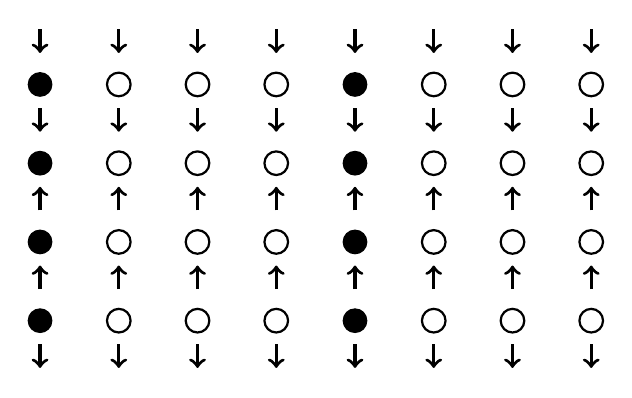
\begin{tikzpicture}
    % charge stripe
    \foreach \y in {0,1,2,3} {
        \foreach \x in {0,4} {
            \filldraw (\x+0,\y) circle [radius=0.15];
            % afm
            \draw [thick] (\x+1,\y) circle [radius=0.15];
            \draw [thick] (\x+2,\y) circle [radius=0.15];
            \draw [thick] (\x+3,\y) circle [radius=0.15];
        }
    }
    
    \foreach \x in {0,1,2,3,4,5,6,7} {
        \draw [very thick, <-] (\x,-0.6) -- (\x,-0.3);
        \draw [very thick, ->] (\x,-0.6+1) -- (\x,-0.3+1);
        \draw [very thick, ->] (\x,-0.6+2) -- (\x,-0.3+2);
        \draw [very thick, <-] (\x,-0.6+3) -- (\x,-0.3+3);
        \draw [very thick, <-] (\x,-0.6+4) -- (\x,-0.3+4);
    }
\end{tikzpicture}
    \caption[2D phonon anomaly sketch]{Possible 2D real-space scenarios of a coupling between the Cu-O bond-stretching phonon at $q=(0.25,0.25,0)$ and stripe order. Here, the phonon wavector is perpendicular to the stripe direction (parallel to the stripe propagation vector). Small arrows represent displacement of oxygen atoms. Charge oscillations are phason modes of the stripes and the black bars represent charge domain walls. The Lower figure refers to a situation where static charge order lowers the energy of the phonon (intuitively through the change of spring constant). open circles represent hole-poor anti-ferromagnetic Cu atoms and filled circles represent hole-doped ($\frac{1}{2}$ hole per site) Cu atoms.}
    \label{fig:anomaly_1d}
\end{figure}

\begin{figure}
    \centering
    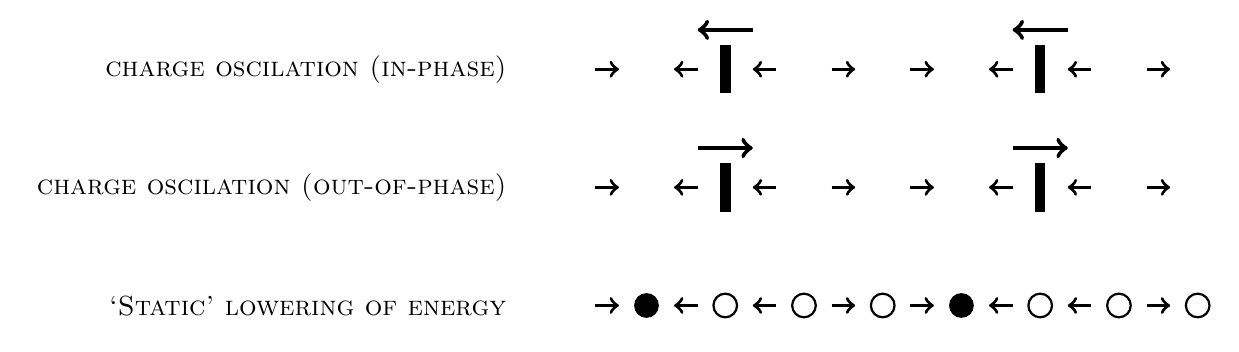
\begin{tikzpicture}
    % domain wall movement
    \foreach \y in {1.5,3} {
        \foreach \x in {0,4} {
            \draw [->, very thick] (\x,\y) -- (\x+0.3,\y);
            \draw [<-, very thick] (\x+1,\y) -- (\x+1.3,\y);
            \draw [<-, very thick] (\x+2,\y) -- (\x+2.3,\y);
            \draw [->, very thick] (\x+3,\y) -- (\x+3.3,\y);
        }
    }
    % domain walls
    \filldraw (1.59, 1.2) rectangle (1.71, 1.8);
    \draw [->, ultra thick] (1.3,2.0) -- (2.0,2.0);
    \filldraw (1.59+4, 1.2) rectangle (1.71+4, 1.8);
    \draw [->, ultra thick] (1.3+4,2.0) -- (2.0+4,2.0);
    \filldraw (1.59+4, 1.2+1.5) rectangle (1.71+4, 1.8+1.5);
    \draw [<-, ultra thick] (1.3,2.0+1.5) -- (2.0,2.0+1.5);
    \filldraw (1.59, 1.2+1.5) rectangle (1.71, 1.8+1.5);
    \draw [<-, ultra thick] (1.3+4,2.0+1.5) -- (2.0+4,2.0+1.5);
    
    % charge stripe
    \foreach \x in {0,4} {
        \draw [->, very thick] (\x,0) -- (\x+0.3,0);
        \draw [<-, very thick] (\x+1,0) -- (\x+1.3,0);
        \draw [<-, very thick] (\x+2,0) -- (\x+2.3,0);
        \draw [->, very thick] (\x+3,0) -- (\x+3.3,0);
        % charge
        \filldraw (\x+0.65,0) circle [radius=0.15];
        % afm
        \draw [thick] (\x+1.65,0) circle [radius=0.15];
        \draw [thick] (\x+2.65,0) circle [radius=0.15];
        \draw [thick] (\x+3.65,0) circle [radius=0.15];
    }
    
    \node [left] at (-1,0) {\textsc{`Static' lowering of energy}};
    \node [left] at (-1,1.5) {\textsc{charge oscilation (out-of-phase)}};
    \node [left] at (-1,3.0) {\textsc{charge oscilation (in-phase)}};
\end{tikzpicture}
    \caption[1D phonon anomaly sketch]{Possible 1D (Kohn Anomaly) scenario of the phonon anomaly. In this case the phonon wavevector resonates with the charge component parallel to the the stripes (perpendicular to the stripe propagation vector).}
    \label{fig:anomaly_2d}
\end{figure}

\begin{figure}
    \centering
    \includegraphics[width=0.7\textwidth]{fig/anomaly/overview.png}
    \caption[Crystal structure annotated with phonon at (0.25,0.25,0) and stripe order]{Sketch of crystal LSCO+O crystal structure containing two distinct dopants in a $4 \times 2 \times 1$ orthorhombic unit cell. The two singular Sr/O dopants correspond to a hole doping of $n_h = \frac{3}{32} \approx 0.09$. Dark blue are magnetic Cu sites while light blue represents hole-rich Cu sites. This period-4/8 segregation into charge/magnetic regions is known as stripe formation \cite{Tranquada1995}. Inset: Possible matching of stripe dynamics with the Cu-O bond stretching mode at q=$(0.25,0.25,0)$ as proposed by \citeauthor{Kaneshita2002} \cite{Kaneshita2002}.}
    \label{fig:crystal_anomaly}
\end{figure}

\begin{figure}
    \centering
    \includegraphics[width=0.54\textwidth]{fig/anomaly/data_reduction.pdf}
    \includegraphics[width=0.45\textwidth]{fig/anomaly/spurion.pdf}
    \caption[IMPS data reduction and Spurion vizualisation]{\textbf{Top-left:} Raw data (summed from one constant-$Q$ scan) from the IMPS 2D detector. The phonon signal is observed in the central area and spurious signal is seen towards the edges. Broken white lines mark the areas used for data reduction. \textbf{Bottom-left:} Result of data reduction using the defined areas. We are clearly able to separate the phonon and spurious signal with this procedure. \textbf{Top-Right:} Scattering triangle responsible for the A-type spurious scattering (broken lines) at $Q=(4.7,4.7,0)$. The culprit is the (8,4,0) reflection. \textbf{Bottom-right:} Simulated effect of the (8,4,0) reflection on a $Q$-$\hbar\omega$ map assuming a Gaussian spurious signal depending on distances in $Q$. Broken line represents a `normal' (not anomalous) dispersion in this region.}
    \label{fig:imps_data_reduction}
\end{figure}

\begin{figure}
    \centering
    \includegraphics[width=0.49\textwidth]{fig/anomaly/selected.pdf}
    \includegraphics[width=0.49\textwidth]{fig/anomaly/disp_aa_2.pdf}
    \caption[Phonon anomaly data and dispersion]{\textbf{Left:} Raw data for LSCO6+O and LCO+O obtained with IMPS detector at IN8, ILL. Fits to Gaussian lineshape. \textbf{Right:} (A) Dispersion of LSCO6+O and LCO+O obtained from peak positions of the raw data. (B) Comparison of the anoamly amplitude (shaded gray area) between LSCO6+O, LCO+O, LSCO15 ($T_\text{c} \approx \SI{40}{\kelvin}$) and LNSCO ($x=0.12$, insulating).}
    \label{fig:anomaly_rawdata}
\end{figure}

\begin{figure}
    \centering
    \includegraphics[width=0.49\textwidth]{fig/anomaly/chi.pdf}
    \includegraphics[width=0.49\textwidth]{fig/anomaly/field_selected.pdf}
    \caption[LSCO6+O magnetic field effect on fluctuations and phonon]{\textbf{Left:} Imaginary part of the magnetic susceptibility in LSCO6+O as a function of energy transfer, field and temperature. As shown, a field of \SI{3}{\tesla} is sufficient to open a gap in the magnetic excitation spectrum. \textbf{Right:} Raw phonon data at anomalous ($h=4.75$) and normal $h=4.5$ wave vectors as a function of field. Contrary to the magnetic excitation spectrum, the anomalous phonon does not appear to be modified by an applied field.}
    \label{fig:phonon_chi_field}
\end{figure}

\section{Things deleted from paper}

\subsection{PDW Stuff in detail}
As is usual with the cuprates, it is difficult to find a framework that captures all of the experimental evidence. With that in mind, we relate our findings to the concept of intertwined orders, while keeping in mind that oxygen-doped samples are macroscopically phase seperated. Intertwined orders are described with reference to pair-density-wave (PDW) superconductivity as the parent microscopic order from which $d$-wave superconductivity, magnetic order, charge order and others emerge\cite{Fradkin2015}. The PDW formalism predicts simultaneous ordering temperatures, gapless magnetic excitations\cite{Christensen2016} and an `electronic liquid crystal' phase\cite{Kivelson1998} that emerges from transverse fluctuations in the charge-density-waves (CDW) of neighbouring stripes. These fluctuations then become the fundamental degrees of freedom relevant to superconductivity. This is consistent with the fact that we see the phonon anomaly whenever the CDW is present, regardless of the nature of the transverse fluctuations. This could potentially explain the `sharper' phonon anomaly in static stripe-ordered LNSCO (Figure DISPERSION)\todo{Note that I have never seen Reznik or Tranquada imply this connection, so it might be a bit too speculative?}.

Returning to LCO+O, LSCO6+O and LSCO15, this would explain the discrepancy in magnetic signatures while still having similar $T_\text{c}$ and phonon anomaly, if we assume that the magnetic domains between the fluctuating stripes can be tuned separately\todo{not sure if this is the case, but in the original papers, electronic liquid phase is described without considering magnetism}. In the case of static charge order and magnetism, this is not the case\cite{Christensen2014}. Another scenario is one in as sample without separate domains of static and fluctuating stripes in which the magnetic field only modifies spectral weight at low energies while not affecting the phonon mode at $\approx 80\,\text{meV}$. A measurement of the phonon anomaly in field of static stripe ordered LSCO ($x=0.12$) would help resolve these issues. A significant disceprency in this interpretation is that fact that LSCO+O is macroscopically phase separated, so the question remains if the two phases are entirely segregated or if exactly one of them contains the physics described here\todo{Linda can you weigh in?}.

\subsection{Chemical disorder - not sure if relevant}
It has been suggested that the inhomogeneous charge distribution due to dopant ions can cause a renormalization of elementary excitations\cite{Park2011}. By adding optimally superconducting, oxygen-doped samples to the list of samples with strong phonon anomalies, we rule out any connection between the phonon anomaly and specific dopant disorder.

\subsection{Discussion}
The results of our measurements (Figure DISPERSION) clearly show the similarity of anomalous behavior between optimally doped LSCO15 and oxygen-overstoichiometric L(S)CO+O. Due to the difference in dopant species, we believe that an immediate result of these measurements is a confirmation of the relationship between fluctuating charge order in the CuO$_2$ planes and the giant phonon anomaly as proposed by \citeauthor{Reznik2012}\cite{Reznik2012}. In the following discussion, we work under the hypothesis that fluctuating charge order in LSCO15 and L(S)CO+O is expressed in the same way despite the different chemistries and bulk characteristics of the two compounds. We start by reviewing some important results from LSCO literature.

It is well established that stripe order is ubiquitous in the cuprates, but a correlation with superconductivity remains elusive and maintaining an internal consistency between measurements is challenging. Neutron scattering, $\mu$SR, NQR and NMR experiments of $T_m$ have shown that static magnetic stripes in LSCO appear at $x=0.03$, take a maximum at $x=0.125$ (where $T_\text{c} \approx 25$ has a minimum) before disappearing abruptly\cite{Julien2003, Hirota2001}. In contrast dynamic magnetic stripes have been observed throughout the superconducting dome, with a gap opening in the spin excitation spectrum for $0.125 < x < 0.20$\cite{Kofu2009, Lee2000, Gilardi2004}. On the other hand, samples considered in this letter both exhibit static magnetic stripes\todo{REF?}, have a gap of 3 meV (LSCO+O)\todo{REF?} and no gap (LCO+O)\cite{Wells1997, Jacobsen2018}, while sharing an optimal $T_\text{c} \approx 40\,\text{K}$. With these results in mind, it is natural to question a trivial relationship between static and dynamic magnetic stripes. Recent measurements by \citeauthor{Jacobsen2018} on LCO+O show a discrepancy in the momentum-transfer of static and dynamic magnetic stripes\cite{Jacobsen2018}, directly showing that the perceived connection might be coincidental.

If the magnetic signal from stripes occur with a modulation of $\delta_\text{m}$, the charge component appears with a modulation of $\delta_\text{c} = 2\delta_\text{m}$. In LSCO static charge stripes have been found for a narrow range of doping ($0.12 < x < 0.13$)\cite{Thampy2014, Croft2014} at the expected position with $\delta_\text{c} = 0.25$. In addition, the static magnetic and static charge stripes have an identical response to magnetic field in LSCO ($x=0.12$) below $T_\text{c}$, indicating a strong connection between the two phenomena\cite{Christensen2014}. Dynamic charge order has, to our knowledge, never been directly observed in LSCO.

Despite the experimental inconsistencies outlined above, we believe that unifying observations of stripe order would be a significant step in our quest to understand superconductivity in the cuprates. The nature of dynamic charge order is a significant missing piece in the stripe picture. The `giant' phonon anomaly observed in LBCO, LSCO, YBCO and now L(S)CO+O represents significant progress in finding said piece. While phonon anomalies, in general, can happen for a number of reasons, the connection to stripe order comes in multiple flavours\cite{Reznik2012}. First, the phonon anomaly obeys the symmetry of charge stripes appearing at $\delta_\text{c} \approx 0.25$. The 1D nature of the phonon anomaly is verified from experiments showing a disappearance of the phonon anomaly by deviating slightly from the Cu-O bond direction\todo{REF?}. ARPES and Inelastic X-ray Scattering (IXS) experiments on LSCO ($x=0.20$)\cite{Park2014} have shown that the phonon anomaly cannot be caused by Fermi Surface nesting (Kohn anomaly). Theoretically, it has been proposed that the phonon anomaly can be explained as steeply dispersing charge fluctuations intersecting the optical phonon branch\cite{Kaneshita2002}

Perhaps the most appealing feature of the phonon anomaly is the apparent correlation with $T_\text{c}$. In LSCO ($x=0.20$ and $x=0.15$), the anomaly amplitude is larger than for samples outside or on the edge of the superconducting dome. The samples studied in this letter follow this trend by having slightly larger $T_\text{c}$ and anomaly amplitudes compared to their LSCO15 cousin.

With this in mind, we believe that the results contained in Figure \ref{fig:dispersion} proves the hypothesis of \citeauthor{Reznik2012} \cite{Reznik2012} that the phonon anomaly is connected to charge fluctuations in the CuO$_2$-planes. Our samples are chemically distinct to LSCO15 and each other, but exhibit identical behavior in terms of the energy scale of the phonon dispersion and the anomaly amplitude. The lack of field effect in Figure FIELD is surprising, but consistent with results on YBCO\todo{REF?}. On the other hand, the phonon anomaly has almost no temperature dependance, indicating that the fluctuations are extremely robust.

\subsection{Old stuff 1}
In addition, the magnitude of this gap $E_g$ has been suspected to track $T_\text{c}$ through the relation $T_c = 1.5 E_\text{g}/k_\text{B}$\cite{Kofu2009}. The samples considered in this letter contradicts this suspicion by having comparable $T_\text{c} \approx 40\,\text{K}$, while LCO+O exhibits no gap\cite{Jacobsen2018,Wells1997} while LSCO+O has a gap of $E_g \approx 3.5$ meV, similar to LSCO15\cite{Lee2000}.


The controversy is rooted in the fact that static stripe order appears to suppress superconductivity while their fluctuations have been proposed to promote superconductivity. It thus becomes natural to ask if the static and dynamic stripe order arises from the same electronic phenomenon and if they are separate phases that can be tuned individually. 

In either case, stripe order has manifestations of competing orders. A notorious example is the `$T_\text{c}$ anomaly' in LSCO, where a suppression of $T_c$ happens at $n_h=\frac{1}{8}$ along with measurable static magnetic and charge order\cite{Christensen2014,Croft2014,Thampy2014}, which is not present in optimally doped LSCO15. In non-superconducting, tetragonal LNSCO and LBCO, similar features have been observed\cite{Wilkins2011}. In addition, \citeauthor{Christensen2014} have shown, by performing experiments in magnetic fields, that the static charge and spin order is connected\cite{Christensen2014}.

Fluctuating magnetic order has been extensively studied throughout the LSCO phase diagram, revealing a connection between 1) the incommensurate modulation $\delta$ of the antiferromagnetic parent phase and 2) the hole doping $n_h$. $\delta$ is equal to $n_h$ up to a saturation at $\delta = n_h = \frac{1}{8}$[yamada], once again stressing the ubiquity of this `$\frac{1}{8}$ phase' in the cuprates.

A playground for understanding this `zoo' of orders is the LSCO+O system, which separates\cite{Mohottala2006} into distinct magnetic ($n_h=\frac{1}{8}$) and superconducting phases\cite{Udby2013}. In addition, the mobile nature of the dopants severely reduces flux pinning\cite{Mohottala2008}, indicating that annealed disorder allows the superconducting part of the sample to emerge in a cleaner way.

From the $T_c$ anomaly in LSCO, phase separation in LSCO+O, the incommensurability $\delta$ of magnetic fluctuations and the insulating nature of LNSCO and LBCO12, we believe that the `$\frac{1}{8}$ phase' is a necessary, but not sufficient precursor for superconductivity. The question then remains: How are the magnetic and charge fluctuations related to this phase and how are they expressed in experiments?

An appealing picture that unite these features is one of simultaneous structural and electronic phase separation in real space, with 1) the $\frac{1}{8}$ non-superconducting phase  expressed by static order and 2) the superconducting phase containing fluctuating charge and magnetic order. Due to the quenched disorder of LSCO this separation only becomes apparent around $n_h = \frac{1}{8}$, while the annealed disorder in LSCO+O results in detectable phase separation at optimal doping.

While subtle, several experiments support this picture. \citeauthor{Kofu2009} reports a different origin of spin fluctuations in LSCO around the $\frac{1}{8}$ anomaly ($x=0.125,0.13.0.135$) above and below a spin gap at $\approx 4$ meV through detailed measurements of the intrinsic linewidth of the excitations. Recently \citeauthor{Jacobsen2018}\cite{Jacobsen2018} reported a different origin in momentum space of the static and dynamic spin stripes through high-resolution measurements of the incommensurability $\delta$ in LCO+O (The same sample studied in this letter). 

Real-space structural phase separation in LCO+O has been probed by X-ray micro-diffraction. \citeauthor{Poccia2012} showed a spatial anti-correlation between two kinds of oxygen orderings\cite{Poccia2012} and in the single-layered cuprate HBCOO ($T_c = 95\,\text{K}$) containing oxygen interstitials, \citeauthor{Campi2015} found a nano-scale spatial anti-correlation between Oxygen-rich and CDW-rich regions\cite{Campi2015}.

We hypothesize that novel charge fluctuations contain vital elements of the pairing mechanism in cuprates, but that SC only arises when the stripe phase is realized locally. In this picture charge fluctuations survive above $T_c$, but SC is realized only as we approach static stripe order.

Starting from our assumption that the phonon anomaly is an expression of steeply dispersing charge fluctuations intersecting an optical phonon branch\cite{Kaneshita2002}, the above picture explains the difference between LSCO15, LNSCO and L(S)CO+O. LNSCO is close to superconductivity, but the specific local structure induced by the addition of Nd$^3+$ ions prevents the `good' charge fluctuations to separate from the $\frac{1}{8}$ phase. The stronger local energetics due to structure produces a steeper dispersion, resulting in a strongly peaked anomaly at $h=\frac{1}{4}$ (charge component of $\frac{1}{8}$ phase). LSCO15 and L(S)CO+O, on the other hand, have an optimal local structure allowing superconductivity to emerge unscathed. The slightly better superconducting properties of the oxygen-overstoichiometric samples are thus reflected in the broader and stronger anomalies. This is also consistent with the experiments performed by \citeauthor{Park2014}\cite{Park2014}, where the strength of the anomaly is found to scale with $T_c$.

Finally, even though we are able to populate the $\frac{1}{8}$ phase with a magnetic field in LSCO+O (Udby et al, to be published) the charge fluctuations connected to SC are completely untouched by a field of 10T ($\ll H_{c2}$) and this is reflected in the absence of modifications of the anomaly (See Figure FIELD).

\chapter{Electronic structure of LSCO+O (ARPES)}
\chapter{Local structure of LSCO+O due to interstitial oxygen (PDF, XAS)}

\begin{framed}
	\begin{itemize}
		\item PDF measurements. Presentation of data. Extraction of distributions (Cu-Oeq).
		\item Superstructure single-crystal measurements
		\item Comparison with simulation.
		\item Why is this structural problem hard? Is it important?
		\item Discussion: Is this impossible to explain with relatively small simulation cells?
		\item Outlook: Classical MD/RMC?
	\end{itemize}
\end{framed}

\section{Data}

\begin{figure}[H]
    \centering
    \includegraphics[width=\textwidth]{fig/pdf/quenched_annealed.pdf}
    \caption{Difference between quenched and annealed cooling procedures for LCO+O and LSCO3+O samples. The topmost plots are comparisons of the reduced and corrected $\text{d}\sigma/\text{d}\omega$ in absolute units, while the difference curves are extracted from the raw $\bm{q}$ data.}
    \label{fig:difference}
\end{figure}

\begin{figure}[H]
    \centering
    \includegraphics[width=\textwidth]{fig/pdf/sample_comparison.pdf}
    \caption{Comparison of the different samples at \SI{300}{\kelvin} in both real and reciprocal space.}
    \label{fig:sample_comparision}    
\end{figure}

\begin{figure}[H]
    \centering
    \includegraphics[width=\textwidth]{fig/pdf/temperature_comparison.pdf}
    \caption{Comparison of \SI{300}{\kelvin} and \SI{15}{\kelvin} for LCO+O and LSCO3+O in both real and reciprocal space.}
    \label{fig:temperature_comparision}    
\end{figure}

\begin{figure}[H]
    \centering
    \includegraphics[width=\textwidth]{fig/pdf/medium_range_pdf.pdf}
    \caption{Short range PDF for all samples at \SI{300}{\kelvin} and \SI{15}{\kelvin}.}
    \label{fig:medium_range_pdf}    
\end{figure}

\begin{figure}[H]
    \centering
    \includegraphics[width=\textwidth]{fig/pdf/cu_o_fits.pdf}
    \caption{Cu-O distance Gaussian fits.}
    \label{fig:cu_o_fits}
\end{figure}

\begin{table}[H]
    \centering
    \begin{tabular}{llll}
        \toprule
          Sample & Temperature [K] &        Cu-O distance [\AA] &           Cu-O $\sigma$ [\AA] \\
        \midrule
             LCO &         300 &  1.9010 $\pm$ 0.0003 &  0.0919 $\pm$ 0.0010 \\
           LCO+O &         300 &  1.9010 $\pm$ 0.0012 &  0.1024 $\pm$ 0.0054 \\
         LSCO3+O &         300 &  1.8995 $\pm$ 0.0003 &  0.0971 $\pm$ 0.0012 \\
           LCO+O &          15 &  1.8983 $\pm$ 0.0009 &  0.1099 $\pm$ 0.0048 \\
         LSCO3+O &          15 &  1.8945 $\pm$ 0.0003 &  0.0987 $\pm$ 0.0012 \\
        \bottomrule
    \end{tabular}    
    \caption{Cu-O distances in all samples at all available temperatures.}
    \label{tab:cu_o_fits}
\end{table}

\begin{figure}[]
    \centering
    \includegraphics[width=\textwidth]{fig/pdf/pdf_simulation_experiment_compare.pdf}
    \caption[PDF data compared with MD simulation]{PDF data compared with MD simulation}
    \label{fig:pdf_sim_comparision}
\end{figure}
\include{ch/discussion}
\chapter{Conclusion}\label{ch:conclusion}
In this chapter, I will attempt to condense the thesis as a whole in order to discuss what was learned through the process of the various experimental and theoretical exercises. In a broad sense, the objective of this thesis is to investigate the effects of chemical disorder through different dopant species in La$_2$CuO$_4$ as introduced in chapter \ref{ch:intro} with the methods presented in chapter \ref{ch:method}. This was primarily done through DFT simulations being compared to a neutron scattering experiment. The challenge with this objective is that we know that the exact electronic structure of the cuprates, at the relevant doping levels, is an unsolved problem in condensed matter. DFT, in particular, has not been very successful in the underdoped part of the phase diagram and many-body methods are usually necessary to explain phenomena such as stripe order and fermi arcs.

\begin{figure}
    \centering
    \includegraphics[width=\textwidth]{fig/conclusion/stripe_electronic_structure.png}
    \caption{Schematic of the electronic structure as a function of hole doping $n_\text{h}$. As one moves from left to right, $n_\text{h}$ increases. On the left we have the undoped compound where there is a gap in electronic density of states due to the antiferromagnetic ground state. As doping is increased, the strong antiferromagnetic interactions are disrupted and novel phenomena such as stripe order and broken Fermi arcs emerge \cite{Keimer2015}. Finally, on the right, the hole doping is sufficient such that the material becomes a normal metal and the strong correlations are destroyed. The electronic band structures are calculated and presented in chapter \ref{ch:simulation}.}
    \label{fig:conclusion_stripe_dft}
\end{figure}

Figure \ref{fig:conclusion_stripe_dft} attempts to visualize this problem by showing how superconductivity is squeezed between localized electrons giving rise to antiferromagnetic order and a fermi liquid with itinerant electrons and a continuous Fermi surface. The solution to this problem was to simply consider the two cases available to us and perform the calculations with this drawback in mind. In some sense, we are trying to figure out how well this level of theory can explain experimental observations. Exactly for this reason, I think a crucial part of this thesis is a careful evaluation of theory with experiment -- essentially we need to know `how wrong' the theory is.

Now, we are certainly not the first to consider La$_2$CuO$_4$ within a one-electron theory. Since DFT was well-established when the high-temperature superconductors were discovered, this methodology was applied right away (see review by \citeauthor{Pickett1989} \cite{Pickett1989}). Various levels of theory have applied to La$_2$CuO$_4$, including pure Hartree-Fock \cite{Su1999}, and semi-local potentials \cite{Lane2018}. Correlated phenomena, such as stripes \cite{Anisimov2004} and broken up Fermi arcs \cite{Lazic2015, Lazic2015a} have even been calculated within DFT, albeit with ad-hoc methods such as DFT+U. 

In this thesis, I make no attempt to contribute to this discussion. Rather, I prioritize getting accurate inter-atomic \emph{forces} such that we get the best possible representation of the phonon spectrum. We thus stick to the generally accepted GGA level of theory. As we saw in chapter \ref{ch:simulation}, some experimentation lead us to the PBESol functional and a significantly increased plane-wave cutoff in order to get reasonable acoustic phonons. 

Within this framework, it was possible to get a good description of the unstable modes related to the structural phase transitions observed in La$_2$CuO$_4$. However, it turns out that the low-temperature tetragonal (LTT) phase is the `most stable' structural phase both with respect to total energy and unstable phonons. Since this LTT phase is known to be suppressing superconductivity, our calculations are consistent with a picture where superconductivity competes with this structural phase and thus prevents the structural phase transition. In this context, I remark that the isostructural, non-superconducting compound La$_2$NiO$_4$ is LTT at low temperatures \cite{Tranquada1994}.

While more experimentation with structural phases, functionals and computational parameters is always desireable, I decided to move on with the relatively successful description of phonon dynamics in La$_2$CuO$_4$ within DFT. In chapter \ref{ch:md}, we use these simulations to approach the actual objective of treating doped La$_2$CuO$_4$ as a defect structure with molecular dynamics. Our analysis of the trajectories show that oxygen interstitials tend towards a LTT-like structure, while undoped and strontium-doped compounds stay LTO-like. While our simulation box and total simulation time is somewhat limited, these results is a good indication of \emph{distinct} dynamics associated with interstitials. Importantly, these distinct dynamics are associated with a modification of the phonon density-of-states which can be observed experimentally.

\section{Oxygen Interstitial Observables}
A large part of this thesis has been dedicated to finding signatures of oxygen interstitials. As mentioned in the introduction, these materials appear to optimize the superconducting transition temperature $T_\text{c}$ and it is suspected that the mobile, interstitial nature might be important for the elevated $T_\text{c}$. As we also show in chapter \ref{ch:local}, the `annealed doping' \cite{Wells1997} associated with interstitial oxygen is mainly observed in diffraction experiments. Remarkably, our high-quality PDF measurement shows almost no signature of oxygen interstitials. The superstructures observed in single-crystal measurements are so strong that this absence must be due to either rotational averaging or because powdered samples simply don't have these superstructures.

However, the dynamics of the \emph{same} powdered samples (measured in chapter \ref{ch:in4}) does have a signature of oxygen interstitials through a broadening of the phonon DOS in the \SIrange{10}{25}{\milli\eV} range. We can qualitatively identify this broadening, through our simulations, as a signature of oxygen disorder. In the case of strontium-doping, on the other hand, we see a sharpening of features which cannot be explained through our simulations. It is possible that the electronic structure of the LSCO $x=0.03$ sample modifies the phonon spectrum in a novel way, but more experiments are required to understand the observations. The fact that we can identify the features in this manner suggests that our model captures some of the dynamics associated with interstitials. This, in extension, is evidence for LTT-like tilts in La$_2$CuO$_{4+\delta}$ in a sample that is always observed to be structurally LTO.

This intimate relationship to an incipient tetragonal phase is also observed in our measurements of soft phonons in chapter \ref{ch:lowen}. While none of these measurements are conclusive on their own, taken together they point to LTT-like behavior being important in La$_2$CuO$_{4+\delta}$ (LCO+O). To briefly recap, I have found that LCO+O features

\begin{enumerate}
    \item LTT-like tilt dynamics.
    \item Instability towards LTT which is stabilized at $T_\text{c}$.
    \item Phase separation into distinct $n_\text{h}=\frac{1}{8}$ and optimally superconducting phases \cite{Mohottala2006,Udby2013}.
\end{enumerate}

\noindent Allowing myself to speculate wildly, this is consistent with a scenario where La$_2$CuO$_{4+\delta}$ is able to optimize the relationship between a stripe phase and a superconducting phase by leveraging LTT-like tilts. In this way, the annealed oxygen order, optimally superconducting phase can be `close' to the static stripe phase without actually being pinned by LTT symmetry. This is consistent with a situation where `stripe degrees of freedom' are necessary for superconductivity, but where we need to be sufficiently far away from static order. Essentially, one could think of a situation where the mobile dopants in La$_2$CuO$_{4+\delta}$ self-organize in a way that optimizes the conditions for these competing orders. A similar idea has been put forward by \citeauthor{Poccia2017} \cite{Poccia2017}, where it is suggested that grain boundaries help optimize this mechanism.

\section{Phonons and Stripes}
The relationship to stripe order in LCO+O was also investigated through measurements of the phonon anomaly in chapter \ref{ch:anomaly}. Contrary to what we saw in the preceding chapters, the phonon anomaly appears to be unrelated to the type of dopant or stripe order. In fact, when reviewing the samples where the phonon anomaly has been observed it appears to be a signature of doping $0.12 < n_\text{h} < 0.20$.

We interpret this as fluctuations of charge stripes, i.e. the stripe degrees of freedom mentioned above. Following the logic from before, this then suggests that charge fluctuations are a necessary but not sufficient condition for optimal superconductivity. In addition, the anomaly persists to high temperatures, so the phenomenon must be intrinsic to the doped samples in a large temperature range.

Very recently, resonant X-ray methods were used to determine `charge density fluctuations' (CDF) in samples of YBa$_2$Cu$_3$O$_{7-\delta}$ and Nd$_{1+x}$Ba$_{2-x}$Cu$_3$O$_{7-\delta}$ over a large doping range. Similar to what has been observed in the phonon anomaly, the CDF's are constrained in the phase diagram, but persists well above the pseudogap temperature $T^*$. Figure \ref{fig:cdw_summary} shows a summary of their results and a schematic of where one finds the phonon anomaly. The similarity of these phenomena strongly supports the suggested \cite{Reznik2012} connection between the phonon anomaly and dynamic stripes.

Finally, we discovered that the electronic structure as observed by ARPES in La$_2$CuO$_{4+\delta}$ is remarkably similar to that of overdoped La$_{1.77}$Sr$_{0.23}$CuO$_4$. Since La$_2$CuO$_{4+\delta}$ is known to phase separate into stripe ordered and superconducting phases, this is interpreted as a superposition of the two phenomena in the ARPES spectrum in chapter \ref{ch:arpes}

\begin{figure}
    \centering
    \includegraphics[width=\textwidth]{fig/conclusion/cdw_summary.png}
    \caption{\textbf{Left:} YBa$_2$Cu$_3$O$_{7-\delta}$ and Nd$_{1+x}$Ba$_{2-x}$Cu$_3$O$_{7-\delta}$ phase diagram showing charge fluctuations in a wide doping/temperature range \cite{Arpaia2019}. \textbf{Right:} Schematic of where the phonon anomaly appears in a generalized cuprate phase diagram (see dicussion in chapter \ref{ch:anomaly}).}
    \label{fig:cdw_summary}
\end{figure}

% \section{Outlook}
% In more concrete terms, I would propose the following research projects:

% \begin{enumerate}
%     \item An extended study of forces in Cuprates using DFT based on our results. Are there other functionals or higher-level theories that might be important in the evaluation of forces. Could include other cuprates to test for generality.
%     \item Classical molecular dynamics of LCO+O. Since DFT limits the size of our simulations box, it could be interesting to construct a large supercell and investigate if the observed superstructures emerge. Forces could be evaluated from the DFT calculations performed here.
%     \item A study of the observed superstructures in La$_2$CuO$_{4+\delta}$ and La$_2$NiO$_{4+\delta}$. Perhaps reverse monte-carlo methods or 2D PDF could be used to solve these structures.
% \end{enumerate}




\appendix

\lstset{basicstyle=\ttfamily\footnotesize, breaklines=true, frame=single}

\chapter{Phonopy tutorial}
In practice, the procedures outlined in this chapter\todo{refer to chapter/section} are sufficiently general such that the calculation of phonon band structures can be performed by a computer program with minimal human interference. In the following example, I will show how phonons are calculated in the HTT phase of LCO using Phonopy and VASP.

\section{Starting Structure}
To begin, you need to know the space group and fractional coordinates of the structure. These are usually determined experimentally through diffraction experiments and can be found in various databases (such as the ICSD [REF?]). For VASP to understand the input structure, it is necessary to convert the downloaded file (usually .cif) into POSCAR format using e.g. VESTA. Since both Phonopy and VASP automatically determines symmetry, the starting structure does not need to be primitive. In this example we use LCO in the orthorhombic coordinate system wth the HTT symmetry (La$_8$Cu$_4$O$_{16}$)

\section{Geometry optimization}
Phonon calculations assumes equilibrium, so it is required to run a geometry optimization in VASP so forces on atoms are minimized prior to displacement generation. There are a few strategies for a successful optimization, see Section XX. Phonon calculations, in general, require accurate forces, so it is recommended to increase the precision significantly. It is typical to set \texttt{EDIFF=1e-8}, \texttt{LREAL=F}, \texttt{PREC=A}, \texttt{ENCUT=800} and to use a mesh density of $\geq 5000$ $k$-points per reciprocal atom. While there is some value in performing the geometry optimization in the supercell used for phonon calculations, this is usually unnecessary and costly in terms of computational time.

\section{Generate displacements}
From the optimized structure, one generates a set of displacements sufficient to populate the dynamical matrix. This is automatically determined by Phonopy and the only user defined parameter is the supercell expansion. Here, we are usually limited by the poor scaling of DFT calculations with respect to system size (effectively $O(n^2 \ln n)$ \footnote{https://scicomp.stackexchange.com/questions/5515/how-does-density-functional-theory-scale-with-system-size}[citation needed]). A typical reasonable size is a few hundred atoms and/or a cube with side length \SIrange{10}{15}{\angstrom}. For this example, we expand the orthorhombic unit cell to a $2 \times 2 \times 1$ super cell with a size of $\SI{10.6}{\angstrom} \times \SI{10.6}{\angstrom} \times \SI{13}{\angstrom}$ and 112 atoms. In order to generate the displacements, one uses the Phonopy command
\begin{lstlisting}
phonopy -c POSCAR -d --dim="2 2 1" --magmom 1 -1 1 -1 0 0 0 0 0 0 0 0 0 0 0 0 0 0 0 0 0 0 0 0 0 0 0 0
\end{lstlisting}

\noindent where \texttt{POSCAR} is the input file. The (optional) \texttt{magmom} tag takes magnetism into account and the 28 numbers correspond to the collinear magnetic moments of each atom. In this example they correspond to the AFM structure of LCO. Including magnetism increases the number of displacements since time-reversal symmetry is broken on neighbouring Cu atoms. The phonopy command generates a number of new \texttt{POSCAR-XXX} files to be used in DFT calculations. In addition, if the magmom tag was specified, a \texttt{MAGMOM} file is generated, providing the magnetic moments of each atom in the supercell.

\section{Run DFT calculations}
One DFT single-point calculation is performed on each of the displaced supercells \texttt{POSCAR-XXX}. Since we are trying to determine forces due to small displacements, high precision is essential. In addition, we can significantly reduce the generated data from the simulation by setting \texttt{LWAVE=F}, \texttt{LCHARG=F}, \texttt{LORBIT=10} and \texttt{LDAUPRINT=0}. The mesh density should be scaled according to the supercell size. In our example we use a $8 \times 8 \times 4$ $k$-point mesh for the original cell and $4 \times 4 \times 4$ for the supercell.

\section{Generate force constants}
Force constants are generated by reading \texttt{vasprun.xml} files from the simulations. The Phonopy command is
\begin{lstlisting}
phonopy -f 01/vasprun.xml 02/vasprun.xml 03/vasprun.xml ...
\end{lstlisting}

\noindent where the \texttt{vasprun.xml} files are listed in the same order as the \texttt{POSCAR-XXX} files that generated them. This procedure generates the force constants, and we have all the information necessary to obtain phonon eigenvalues and eigenvectors.

\section{Saving and Distributing}
At this point, we can generate phonon band structures, density of states, thermodynamic properties and visualize phonon modes. For details, I will refer to the Phonopy website [REF\footnote{https://atztogo.github.io/phonopy/}] and the excellent phonon visualization website [REF\footnote{http://henriquemiranda.github.io/phononwebsite/index.html}]. The data needed to construct the dynamical matrix is fully contained in the \texttt{FORCE\_SETS} and \texttt{phonopy\_disp.yaml} files. While these files are sufficient to distribute phonon data, it is useful to include the computational parameters geometry optimization and phonon calculations.

\chapter{PhononNeutron - Comparing Simulation and Experiment}\label{app:software}
During the thesis, a selection of python classes were developed with the intention of generalizing some of the tasks required to get the correct neutron weights out of simulations. While software such as MDANSE does a good job with respect to molecular dynamics, I wanted something focussed on analysing phonons specifically from different levels of theory (MD and `Frozen Phonons').

The code be found at \url{https://github.com/tejsner/phonon_neutron} along with installation instructions. The intention of this appendix is to explain some of the functionality and to serve as a tutorial for anyone interested in performing the same kind of analysis.

\begin{itemize}
    \item md\_tools.py
    \item phonopy\_tools.py
    \item cuprate.py
\end{itemize}

\chapter{Structural Transformation Matrices}

Conventional Cells (Bmab and P4$_2$/ncm are identical so this transformation is the identity)

\[
\text{I4/mmm} \quad 
\begin{pmatrix}
1 & \bar{1} & 0 \\
1 & 1 & 0 \\
0 & 0 & 1
\end{pmatrix}
\quad \text{Bmab}
\]

\noindent Primitive Cells

\[
\text{I4/mmm} \quad 
\begin{pmatrix}
1 & 1 & 0 \\
1 & \bar{1} & 0 \\
1 & 0 & \bar{1}
\end{pmatrix}
\quad \text{Bmab} \quad
\begin{pmatrix}
1 & 0 & 1 \\
0 & 1 & 0 \\
\bar{1} & 0 & 1
\end{pmatrix} 
\quad \text{P4}_2\text{/ncm}
\]

\chapter{Additional Data}
This appendix contains plots and analysis that would be distracting in the main text, but are important to reference in any thorough investigation.

\chapter{VASP Inputs}\label{app:vasp}

\begin{figure}
    \centering
    \begin{lstlisting}[basicstyle=\footnotesize\ttfamily, frame=single]
    ENCUT = 520 # 1.3x suggested value from O POTCAR, 800 for phonons
    EDIFF = 1E-5 # 1E-8 for phonons
    ALGO = NORMAL
    PREC = Accurate
    ADDGRID = .FALSE.
    LREAL = Auto # Switch to .FALSE. for phonons
    
    GGA = PS # PBESol functional, PE switches to default PBE
    
    ISPIN = 2
    MAGMOM = 1 -1 1 -1 24*0 # AFM structure
    
    IBRION = -1 # Single point calculation
    NSW = 0     # Number of ionic steps
    
    ISMEAR = 0
    SIGMA = 0.1
    
    LDAU= .TRUE. # Enable LDA+U with U=8eV and J=0.8eV
    LDAUTYPE = 4 # No exchange splitting
    LDAUL = 2 -1 -1 # only on Cu d states
    LDAUU = 8 0 0 
    LDAUJ = 0.8 0 0
    \end{lstlisting}
    \caption[VASP: Typical INCAR]{Typical INCAR for VASP simulations.}
    \label{fig:incar}
\end{figure}

\chapter{Low energy phonon additional plots}\label{app:lowen_plots}

\begin{figure}
    \centering
    \includegraphics[width=\textwidth]{fig/lowen/fits_400T.pdf}
    \caption[400T flatcone raw data]{400T flatcone raw data}
    %label{fig:flatcone_phonons_400T_raw}    
\end{figure}

\begin{figure}
    \centering
    \includegraphics[width=\textwidth]{fig/lowen/fits_220T.pdf}
    \caption[220T flatcone raw data]{220T flatcone raw data}
    %\label{fig:flatcone_phonons_400T_raw}
\end{figure}

\begin{figure}
    \centering
    \includegraphics[width=\textwidth]{fig/lowen/fits_400L.pdf}
    \caption[400L flatcone raw data]{400L flatcone raw data}
    %\label{fig:flatcone_phonons_400L_raw}    
\end{figure}

\begin{figure}
    \centering
    \includegraphics[width=\textwidth]{fig/lowen/fits_220L.pdf}
    \caption[220L flatcone raw data]{220L flatcone raw data}
    %\label{fig:flatcone_phonons_220L_raw}    
\end{figure}

\begin{figure}[]
    \centering
    \includegraphics[width=\textwidth]{fig/lowen/flatcone_fits_simulation_htt_afm.png}
    \caption[Flatcone dispersion and neutron weighted simulation data]{Flatcone dispersion and neutron weighted simulation data. HTT AFM simulation data.}
    %\label{fig:flatcone_phonons_dispersion_simulation}
\end{figure}

\begin{figure}[]
    \centering
    \includegraphics[width=\textwidth]{fig/lowen/flatcone_fits_simulation_ltt_afm.png}
    \caption[Flatcone dispersion and neutron weighted simulation data]{Flatcone dispersion and neutron weighted simulation data. LTT AFM simulation data.}
    %\label{fig:flatcone_phonons_dispersion_simulation}
\end{figure}

\begin{figure}[]
    \centering
    \includegraphics[width=\textwidth]{fig/lowen/flatcone_fits_simulation_htt_metal.png}
    \caption[Flatcone dispersion and neutron weighted simulation data]{Flatcone dispersion and neutron weighted simulation data. LTT AFM simulation data.}
    %\label{fig:flatcone_phonons_dispersion_simulation}
\end{figure}

\begin{figure}[]
    \centering
    \includegraphics[width=\textwidth]{fig/lowen/flatcone_fits_simulation_lto_metal.png}
    \caption[Flatcone dispersion and neutron weighted simulation data]{Flatcone dispersion and neutron weighted simulation data. LTO metal simulation data.}
    %\label{fig:flatcone_phonons_dispersion_simulation}
\end{figure}

\begin{figure}[]
    \centering
    \includegraphics[width=\textwidth]{fig/lowen/flatcone_fits_simulation_ltt_metal.png}
    \caption[Flatcone dispersion and neutron weighted simulation data]{Flatcone dispersion and neutron weighted simulation data. LTT Metal simulation data.}
    %\label{fig:flatcone_phonons_dispersion_simulation}
\end{figure}

\chapter{Additional Phonon DOS plots}\label{app:pdos_plots}

\begin{figure}
    \centering
    \includegraphics[width=\textwidth]{fig/gdos/in4_60K.pdf}
    \caption[gDOS at \SI{60}{\kelvin}]{GDOS at \SI{60}{\kelvin}}
    \label{fig:gdos_60k}
\end{figure}

\begin{figure}
    \centering
    \includegraphics[width=\textwidth]{fig/gdos/in4_300K.pdf}
    \caption[gDOS at \SI{300}{\kelvin}]{GDOS at \SI{300}{\kelvin}}
    \label{fig:gdos_300k}
\end{figure}

\bibliographystyle{apsrev4-1}
\bibliography{bibliography}

\end{document}
